\documentclass[11pt]{article}

\usepackage[a4paper,margin=0.75in]{geometry}
\usepackage{amsmath,amssymb}
\usepackage{graphicx}
\usepackage{booktabs}
\usepackage{array}
\usepackage{float}
\usepackage{hyperref}
\usepackage{enumitem}
\usepackage{xcolor}
\usepackage{tikz}
\usetikzlibrary{positioning,arrows.meta,shapes.geometric}

\setlist{nosep}
\renewcommand{\arraystretch}{1.3}

\tikzset{
layer/.style={
draw,
rounded corners,
minimum width=2.2cm,
minimum height=0.9cm,
align=center,
fill=blue!10
},
arrow/.style={
-{Latex[length=3mm]},
thick
}
}

\begin{document}

%%%%%%%%%%%%%%%%%%%%%%%%%%%%%%%%%%%%%%%%%%%%%%%%%%%%%%%%%%%%

\begin{center}

{\Large\textbf{Shiv Nadar University Chennai}}

\vspace{3mm}

{\large\textbf{CS3807 -- Deep Learning Laboratory}}

\vspace{3mm}

{\Large\textbf{Experiment 4}}

\vspace{2mm}

{\Large\textbf{Comparative Study of Deep Convolutional Neural}}

{\Large\textbf{Network Architectures Using Transfer Learning}}

\end{center}

\vspace{5mm}

\begin{tabular}{|p{4cm}|p{8cm}|p{2cm}|}
\hline
Degree \& Branch &
B.Tech Artificial Intelligence \& Data Science &
Semester V\\
\hline
Subject Code \& Name &
CS3807 -- Deep Learning Laboratory &
AY: 2026--27\\
\hline
\end{tabular}

%%%%%%%%%%%%%%%%%%%%%%%%%%%%%%%%%%%%%%%%%%%%%%%%%%%%%%%%%%%%

\section*{1. Objective}

The objectives of this experiment are

\begin{itemize}

\item Study the evolution of deep CNN architectures.

\item Compare LeNet-5, AlexNet, VGG16, GoogleNet and ResNet.

\item Understand transfer learning.

\item Fine tune pretrained CNN models.

\item Compare classification performance of different architectures.

\end{itemize}

%%%%%%%%%%%%%%%%%%%%%%%%%%%%%%%%%%%%%%%%%%%%%%%%%%%%%%%%%%%%

\section*{2. Learning Outcomes}

After completing this experiment students will be able to

\begin{enumerate}

\item Explain modern CNN architectures.

\item Differentiate LeNet, AlexNet, VGG16, GoogleNet and ResNet.

\item Implement transfer learning.

\item Fine tune pretrained CNN models.

\item Compare CNN architectures using performance metrics.

\end{enumerate}

%%%%%%%%%%%%%%%%%%%%%%%%%%%%%%%%%%%%%%%%%%%%%%%%%%%%%%%%%%%%

\section*{3. Introduction}

Deep Convolutional Neural Networks have become the dominant models for
computer vision applications because they automatically learn hierarchical
features from images. The evolution of CNNs has focused on improving
classification accuracy while reducing computational complexity and
training difficulties.

The progression of CNN architectures began with LeNet-5 and has evolved
through AlexNet, VGGNet, GoogleNet, and ResNet. Each architecture
introduced important innovations that significantly improved image
classification performance.

%%%%%%%%%%%%%%%%%%%%%%%%%%%%%%%%%%%%%%%%%%%%%%%%%%%%%%%%%%%%

\section*{4. Evolution of CNN Architectures}

\begin{center}

\begin{tabular}{|c|c|p{7cm}|}

\hline

Model & Year & Major Contribution\\

\hline

LeNet-5 & 1998 &
First practical convolutional neural network\\

\hline

AlexNet & 2012 &
ReLU activation, Dropout and GPU training\\

\hline

VGG16 & 2014 &
Uniform $3\times3$ convolution filters\\

\hline

GoogleNet & 2014 &
Inception modules for multi-scale feature extraction\\

\hline

ResNet & 2015 &
Residual learning using skip connections\\

\hline

\end{tabular}

\end{center}

%%%%%%%%%%%%%%%%%%%%%%%%%%%%%%%%%%%%%%%%%%%%%%%%%%%%%%%%%%%%

\section*{5. LeNet-5}

LeNet-5 was proposed by Yann LeCun in 1998 for handwritten digit
recognition. It consists of two convolution layers, two average pooling
layers and fully connected layers. It demonstrated that convolutional
networks could automatically learn image features without handcrafted
feature extraction.


Advantages

\begin{itemize}

\item Small number of parameters

\item Fast training

\item Suitable for OCR

\end{itemize}

%%%%%%%%%%%%%%%%%%%%%%%%%%%%%%%%%%%%%%%%%%%%%%%%%%%%%%%%%%%%

\section*{6. AlexNet}

AlexNet won the ImageNet Challenge in 2012 by reducing the
classification error significantly. It introduced ReLU activation,
Dropout regularization and GPU training.


Major innovations

\begin{itemize}

\item ReLU activation

\item Dropout

\item GPU implementation

\item Data augmentation

\end{itemize}

%%%%%%%%%%%%%%%%%%%%%%%%%%%%%%%%%%%%%%%%%%%%%%%%%%%%%%%%%%%%

\section*{7. VGG16}

VGG16 demonstrated that using multiple small $3\times3$ convolution
filters could outperform larger filters while increasing network depth.


Advantages

\begin{itemize}

\item Excellent feature extraction

\item Simple architecture

\item High classification accuracy

\end{itemize}

%%%%%%%%%%%%%%%%%%%%%%%%%%%%%%%%%%%%%%%%%%%%%%%%%%%%%%%%%%%%

\section*{8. Comparison of Architectures}

\begin{center}

\begin{tabular}{|l|c|c|c|}

\hline

Architecture &
Depth &
Parameters &
Main Contribution\\

\hline

LeNet-5 &
7 &
60K &
First CNN\\

AlexNet &
8 &
61M &
ReLU + Dropout\\

VGG16 &
16 &
138M &
Deep 3$\times3$ filters\\

GoogleNet &
22 &
6.8M &
Inception Modules\\

ResNet50 &
50 &
25.6M &
Residual Learning\\

\hline

\end{tabular}

\end{center}

% --------- CONTINUE WITH PART 2 ---------
%%%%%%%%%%%%%%%%%%%%%%%%%%%%%%%%%%%%%%%%%%%%%%%%%%%%%%%%%%%%
\section*{9. GoogleNet (Inception Network)}

GoogleNet, proposed by Szegedy \textit{et al.} in 2014, introduced the
\textbf{Inception Module}, which performs multiple convolution operations
in parallel using different filter sizes. Instead of using only a single
kernel size, GoogleNet simultaneously applies $1\times1$, $3\times3$,
$5\times5$ convolutions and max pooling. The outputs are concatenated to
obtain multi-scale feature representations.

The use of $1\times1$ convolutions before larger kernels reduces the
number of trainable parameters and computational complexity.


Advantages

\begin{itemize}
\item Multi-scale feature extraction.
\item Fewer parameters than VGG16.
\item High computational efficiency.
\item Better classification performance.
\end{itemize}

%%%%%%%%%%%%%%%%%%%%%%%%%%%%%%%%%%%%%%%%%%%%%%%%%%%%%%%%%%%%

\section*{10. ResNet}

Increasing CNN depth often causes the \textbf{vanishing gradient problem},
making optimization difficult. ResNet solves this issue using
\textbf{skip (residual) connections}, allowing gradients to flow directly
through the network.

Instead of learning

\[
H(x)
\]

ResNet learns

\[
F(x)=H(x)-x
\]

thus,

\[
Output = F(x)+x
\]

where

\begin{itemize}
\item $F(x)$ = Residual Mapping
\item $x$ = Identity Mapping
\end{itemize}

\begin{figure}[H]
\centering

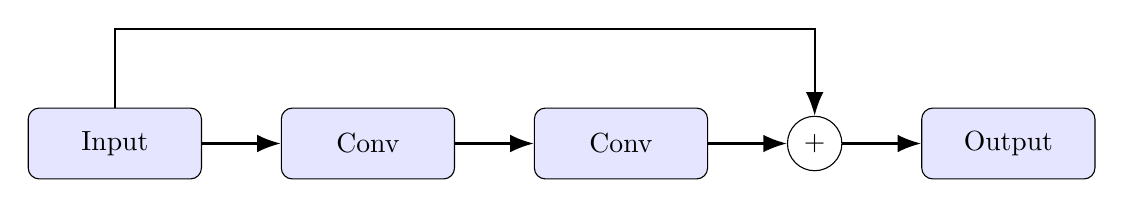
\begin{tikzpicture}[node distance=1cm]

\node[layer](input){Input};

\node[layer,right=of input](conv1){Conv};

\node[layer,right=of conv1](conv2){Conv};

\node[circle,draw,right=of conv2](add){+};

\node[layer,right=of add](output){Output};

\draw[arrow](input)--(conv1);
\draw[arrow](conv1)--(conv2);
\draw[arrow](conv2)--(add);
\draw[arrow](add)--(output);

\draw[arrow]
(input)
|-([yshift=10mm]conv2.north)
-| (add.north);

\end{tikzpicture}

\caption{Residual Block in ResNet}
\end{figure}

Advantages

\begin{itemize}
\item Eliminates vanishing gradients.
\item Enables very deep neural networks.
\item Faster convergence.
\item High ImageNet accuracy.
\end{itemize}

%%%%%%%%%%%%%%%%%%%%%%%%%%%%%%%%%%%%%%%%%%%%%%%%%%%%%%%%%%%%

\section*{11. Dilated Convolution}

Dilated convolution (also called atrous convolution) increases the
receptive field without increasing the number of parameters.

The dilation rate determines the spacing between kernel elements.

For a standard convolution,

\[
D=1
\]

For dilated convolution,

\[
D>1
\]

Example

\[
\begin{bmatrix}
1 & 0 & 2\\
0 & 3 & 0\\
4 & 0 & 5
\end{bmatrix}
\]

where zeros indicate inserted gaps.

Applications

\begin{itemize}
\item Semantic segmentation
\item Medical image analysis
\item Satellite imagery
\item Object localization
\end{itemize}

%%%%%%%%%%%%%%%%%%%%%%%%%%%%%%%%%%%%%%%%%%%%%%%%%%%%%%%%%%%%

\section*{12. Transpose Convolution}

Transpose convolution increases the spatial dimensions of feature maps.
Unlike pooling, which reduces image size, transpose convolution performs
learnable upsampling.

Applications

\begin{itemize}
\item Image Super Resolution
\item Autoencoders
\item GANs
\item Image Generation
\item Semantic Segmentation
\end{itemize}

%%%%%%%%%%%%%%%%%%%%%%%%%%%%%%%%%%%%%%%%%%%%%%%%%%%%%%%%%%%%

\section*{13. Transfer Learning}

Transfer Learning utilizes a pretrained CNN model that has already learned
general image features from a large dataset such as ImageNet.

Instead of training from scratch,

\begin{enumerate}
\item Load a pretrained model.
\item Remove the original classifier.
\item Freeze convolution layers.
\item Add new Dense layers.
\item Train the classifier.
\item Fine tune selected convolution layers.
\end{enumerate}

\begin{figure}[H]

\centering

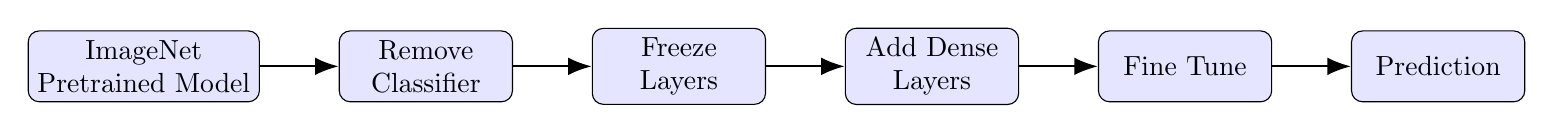
\begin{tikzpicture}[node distance=1cm]

\node[layer](a){ImageNet\\Pretrained Model};

\node[layer,right=of a](b){Remove\\Classifier};

\node[layer,right=of b](c){Freeze\\Layers};

\node[layer,right=of c](d){Add Dense\\Layers};

\node[layer,right=of d](e){Fine Tune};

\node[layer,right=of e](f){Prediction};

\foreach \x/\y in {a/b,b/c,c/d,d/e,e/f}
\draw[arrow](\x)--(\y);

\end{tikzpicture}

\caption{Transfer Learning Workflow}

\end{figure}

Advantages

\begin{itemize}
\item Faster convergence.
\item Higher accuracy on small datasets.
\item Reduced training time.
\item Lower computational cost.
\end{itemize}

%%%%%%%%%%%%%%%%%%%%%%%%%%%%%%%%%%%%%%%%%%%%%%%%%%%%%%%%%%%%

\section*{14. Dataset}

Dataset: CIFAR-10

\begin{itemize}

\item Training Images : 50,000

\item Testing Images : 10,000

\item Number of Classes : 10

\item Image Size : $32\times32\times3$

\item Classes:
Airplane, Automobile, Bird, Cat, Deer,
Dog, Frog, Horse, Ship and Truck.

\end{itemize}

%%%%%%%%%%%%%%%%%%%%%%%%%%%%%%%%%%%%%%%%%%%%%%%%%%%%%%%%%%%%
% Continue with Part 3
%%%%%%%%%%%%%%%%%%%%%%%%%%%%%%%%%%%%%%%%%%%%%%%%%%%%%%%%%%%%

\section*{15. Experimental Procedure}

\subsection*{Task 1: Dataset Preparation}

\begin{enumerate}

\item Load the CIFAR-10 dataset using TensorFlow/Keras.

\item Normalize the pixel values to the range [0,1].

\item Display ten sample images.

\item Print the dimensions of the training and testing datasets.

\end{enumerate}

%%%%%%%%%%%%%%%%%%%%%%%%%%%%%%%%%%%%%%%%%%%%%%%%%%%%%%%%%%%%

\subsection*{Task 2: Transfer Learning}

Load any one of the following pretrained CNN models.

\begin{itemize}

\item VGG16

\item ResNet50

\item MobileNetV2

\item EfficientNetB0 (Optional)

\end{itemize}

Perform the following steps.

\begin{enumerate}

\item Load pretrained ImageNet weights.

\item Remove the original classification layer.

\item Freeze the convolutional base.

\item Add a Global Average Pooling layer.

\item Add a Dense layer with ReLU activation.

\item Add the output layer with Softmax activation.

\end{enumerate}

%%%%%%%%%%%%%%%%%%%%%%%%%%%%%%%%%%%%%%%%%%%%%%%%%%%%%%%%%%%%

\subsection*{Task 3: Model Training}

Train the model using

\begin{center}

\begin{tabular}{|p{5cm}|p{6cm}|}

\hline

Optimizer & Adam\\

\hline

Learning Rate & 0.001\\

\hline

Batch Size & 32\\

\hline

Epochs & 10--20\\

\hline

Loss Function &
Categorical Cross Entropy\\

\hline

Evaluation Metric &
Accuracy\\

\hline

\end{tabular}

\end{center}

%%%%%%%%%%%%%%%%%%%%%%%%%%%%%%%%%%%%%%%%%%%%%%%%%%%%%%%%%%%%

\subsection*{Task 4: Fine Tuning}

\begin{enumerate}

\item Unfreeze the last convolution block.

\item Train for another 5--10 epochs.

\item Compare the classification accuracy before and after fine tuning.

\end{enumerate}

%%%%%%%%%%%%%%%%%%%%%%%%%%%%%%%%%%%%%%%%%%%%%%%%%%%%%%%%%%%%

\subsection*{Task 5: Model Evaluation}

Evaluate the trained model using

\begin{itemize}

\item Accuracy

\item Precision

\item Recall

\item F1-score

\item Confusion Matrix

\item Classification Report

\end{itemize}

%%%%%%%%%%%%%%%%%%%%%%%%%%%%%%%%%%%%%%%%%%%%%%%%%%%%%%%%%%%%

\section*{16. Hyperparameter Study}

Compare the performance using different settings.

\begin{center}

\begin{tabular}{|l|l|}

\hline

Hyperparameter & Values\\

\hline

Learning Rate &
0.001, 0.0001\\

\hline

Batch Size &
16, 32, 64\\

\hline

Epochs &
10, 20\\

\hline

Optimizer &
Adam, SGD\\

\hline

Dense Units &
128, 256\\

\hline

Frozen Layers &
All, Partial\\

\hline

\end{tabular}

\end{center}

%%%%%%%%%%%%%%%%%%%%%%%%%%%%%%%%%%%%%%%%%%%%%%%%%%%%%%%%%%%%

\section*{17. Mandatory Plots}

Include the following plots in the laboratory report.

\begin{enumerate}

\item Sample CIFAR-10 images

\item Training Accuracy

\item Validation Accuracy

\item Training Loss

\item Validation Loss

\item Confusion Matrix

\item Misclassified Images (Optional)

\end{enumerate}

Students should write a brief inference (2--3 lines) for each figure.

\begin{figure}[H]
\centering
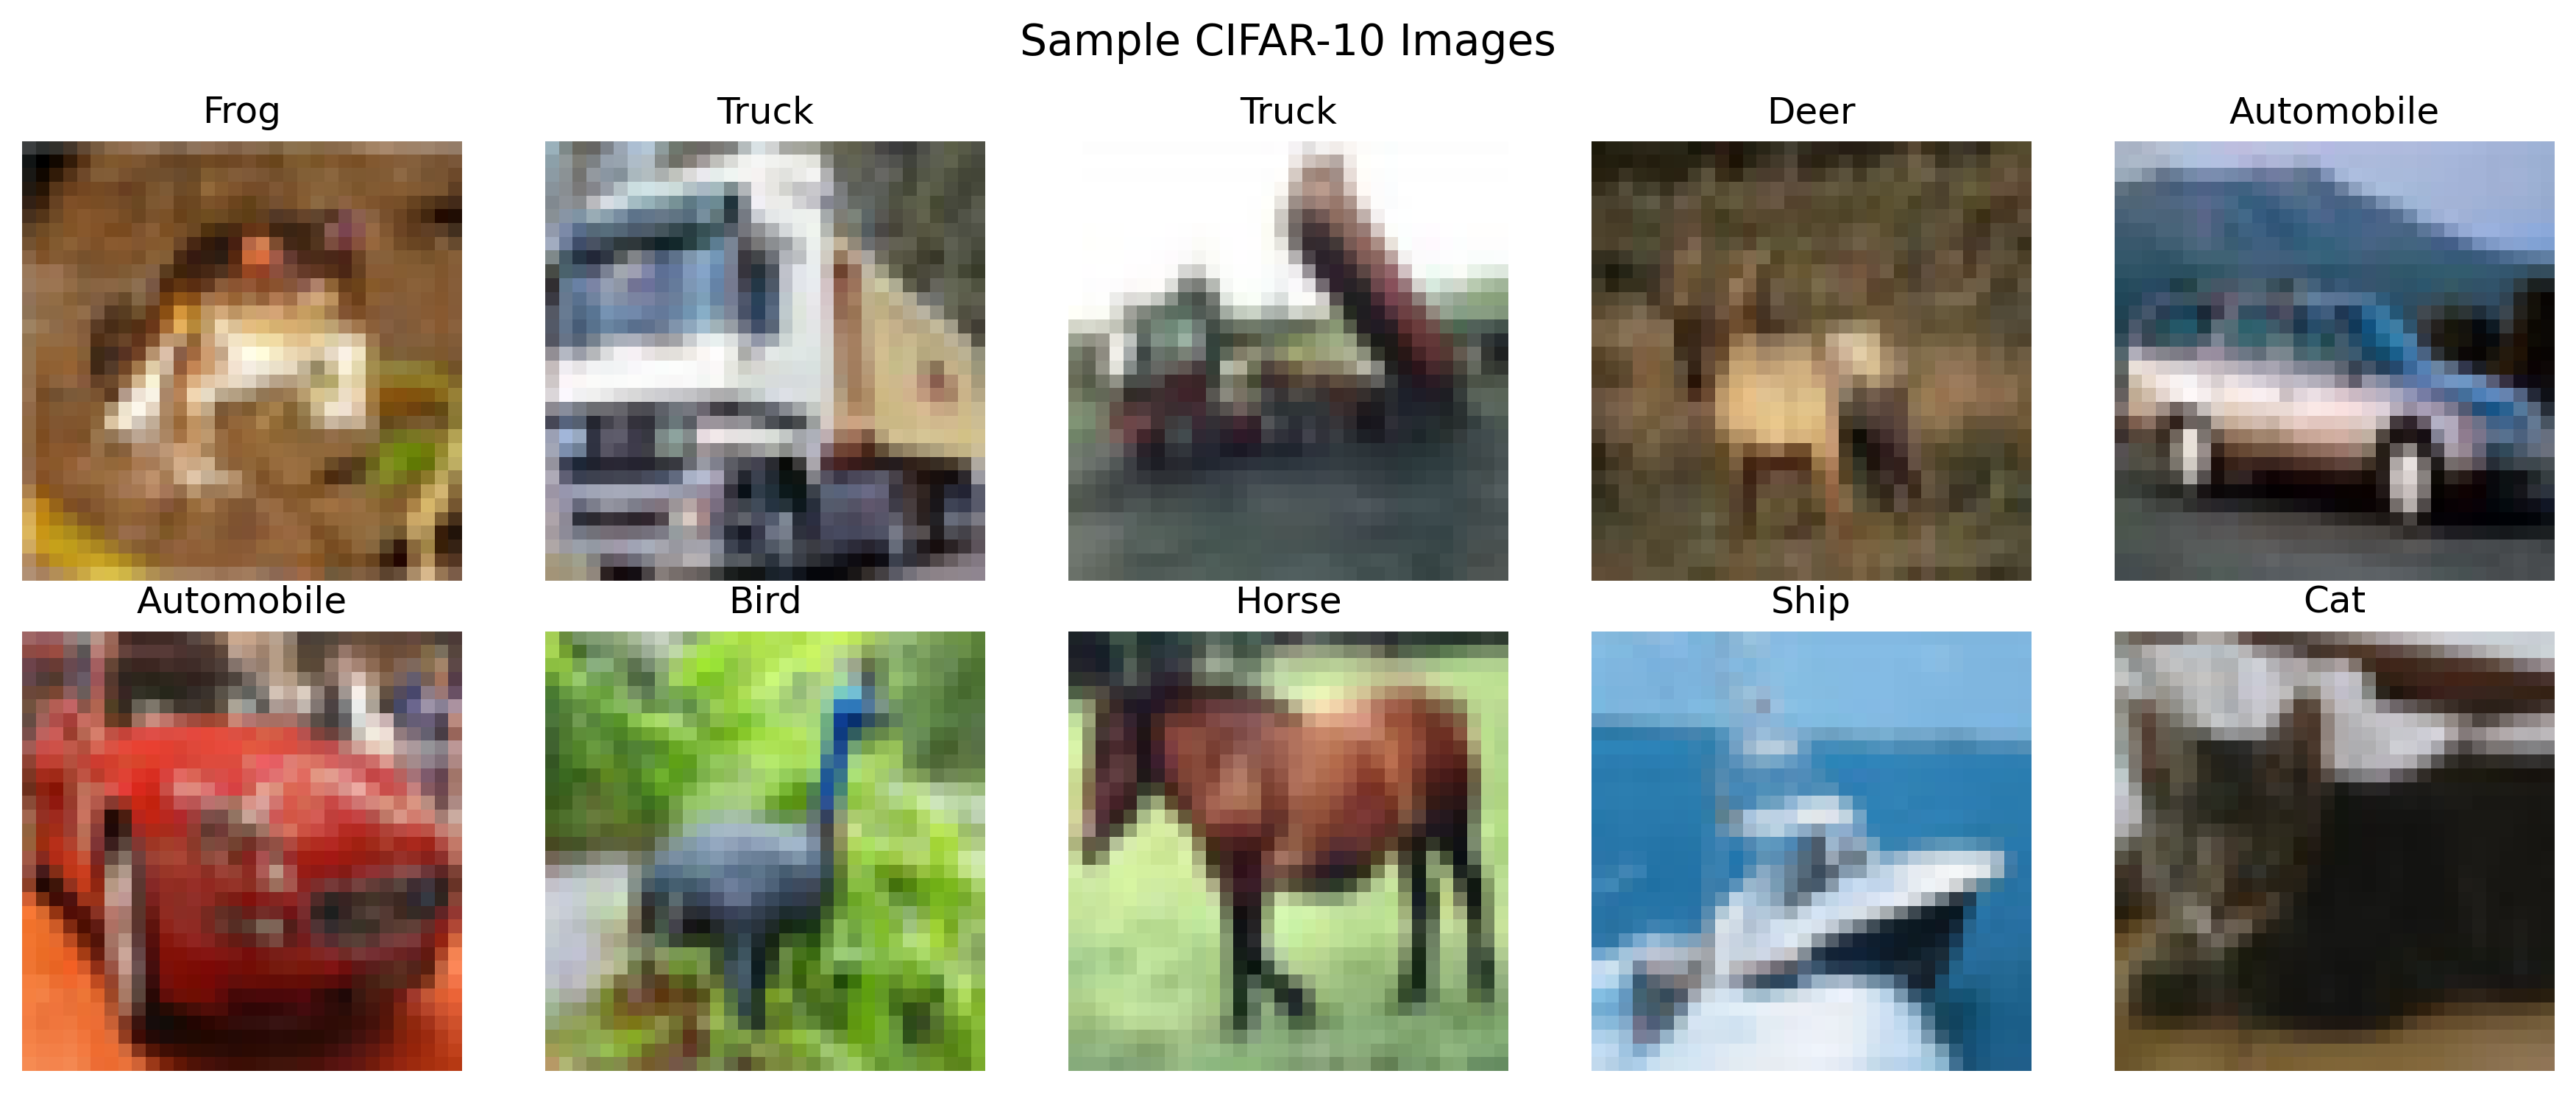
\includegraphics[width=0.75\textwidth]{plots/1_sample_cifar10_images.png}
\caption{Sample CIFAR-10 Images}
\end{figure}

\noindent\textit{Inference:} The figure shows ten representative $32\times32\times3$ images from the CIFAR-10 training set spanning all ten classes. The low resolution and visual similarity between certain classes (e.g., cat vs. dog, automobile vs. truck) illustrate why CIFAR-10 is a non-trivial classification benchmark even for deep pretrained models.

\begin{figure}[H]
\centering
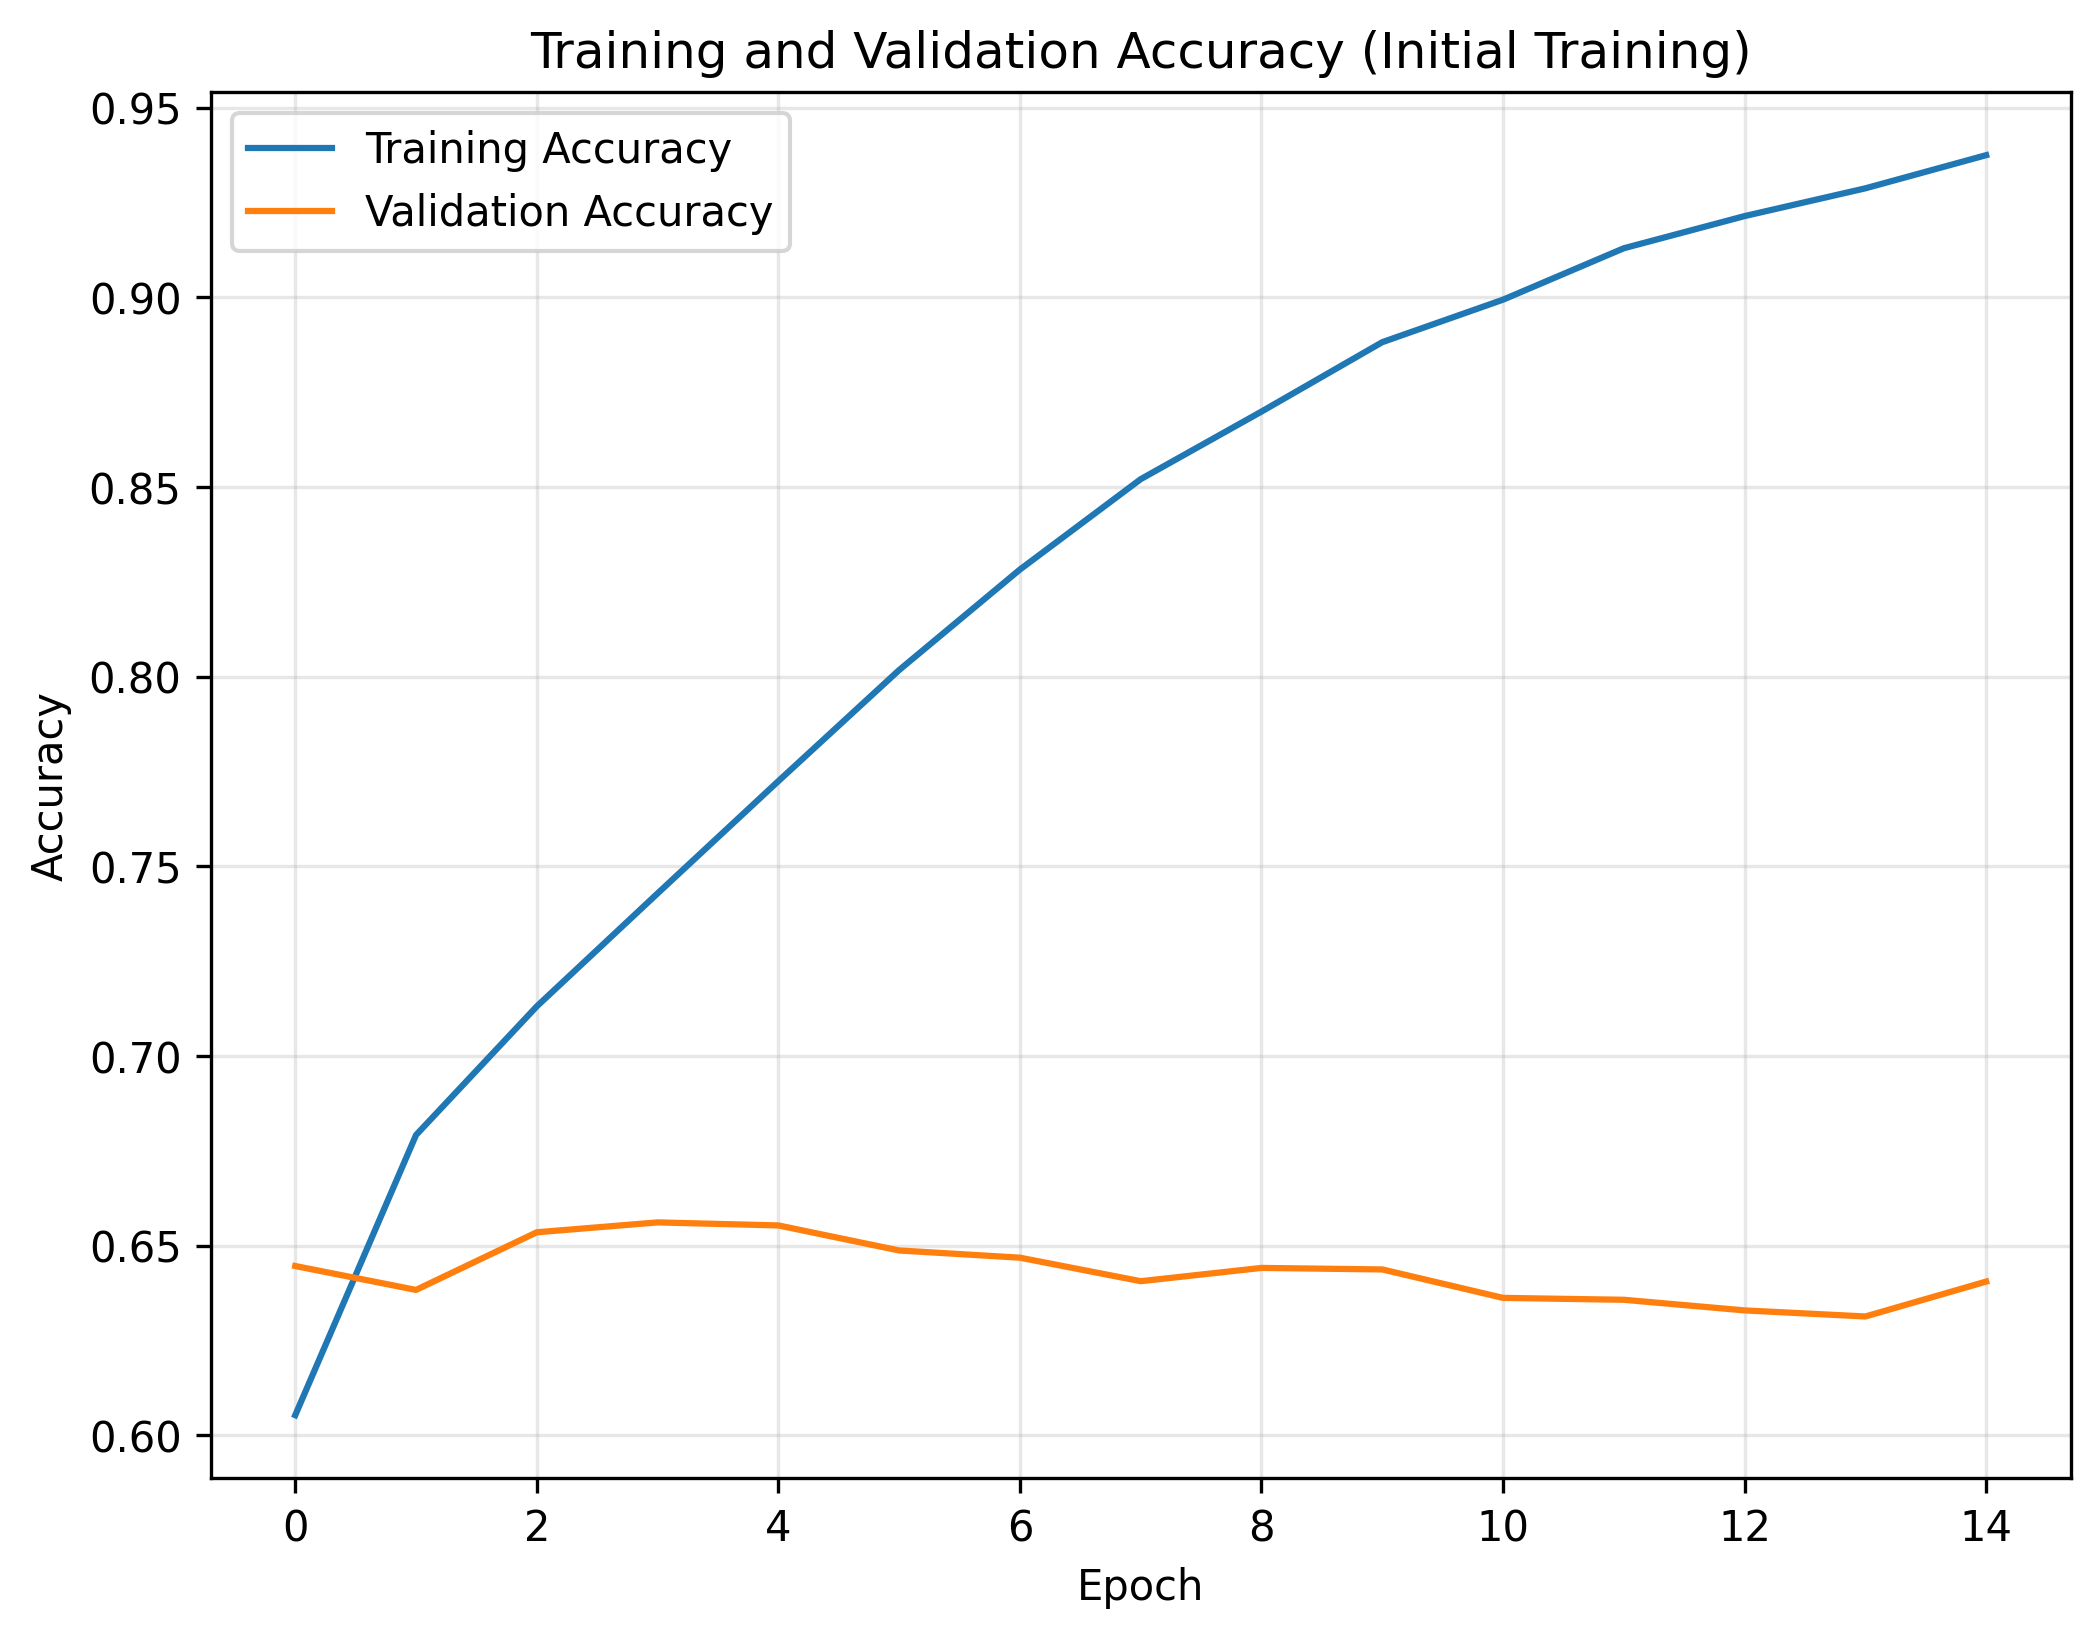
\includegraphics[width=0.7\textwidth]{plots/2_3_training_validation_accuracy.png}
\caption{Training vs Validation Accuracy -- ResNet50 (Initial Training, Frozen Base)}
\end{figure}

\noindent\textit{Inference:} During the initial 15-epoch training phase with the ResNet50 base frozen, training accuracy rose steadily to 93.75\%, while validation accuracy plateaued near 64\%. The widening gap between the curves indicates the frozen convolutional base combined with the classifier head begins to overfit the training data past roughly epoch 5.

\begin{figure}[H]
\centering
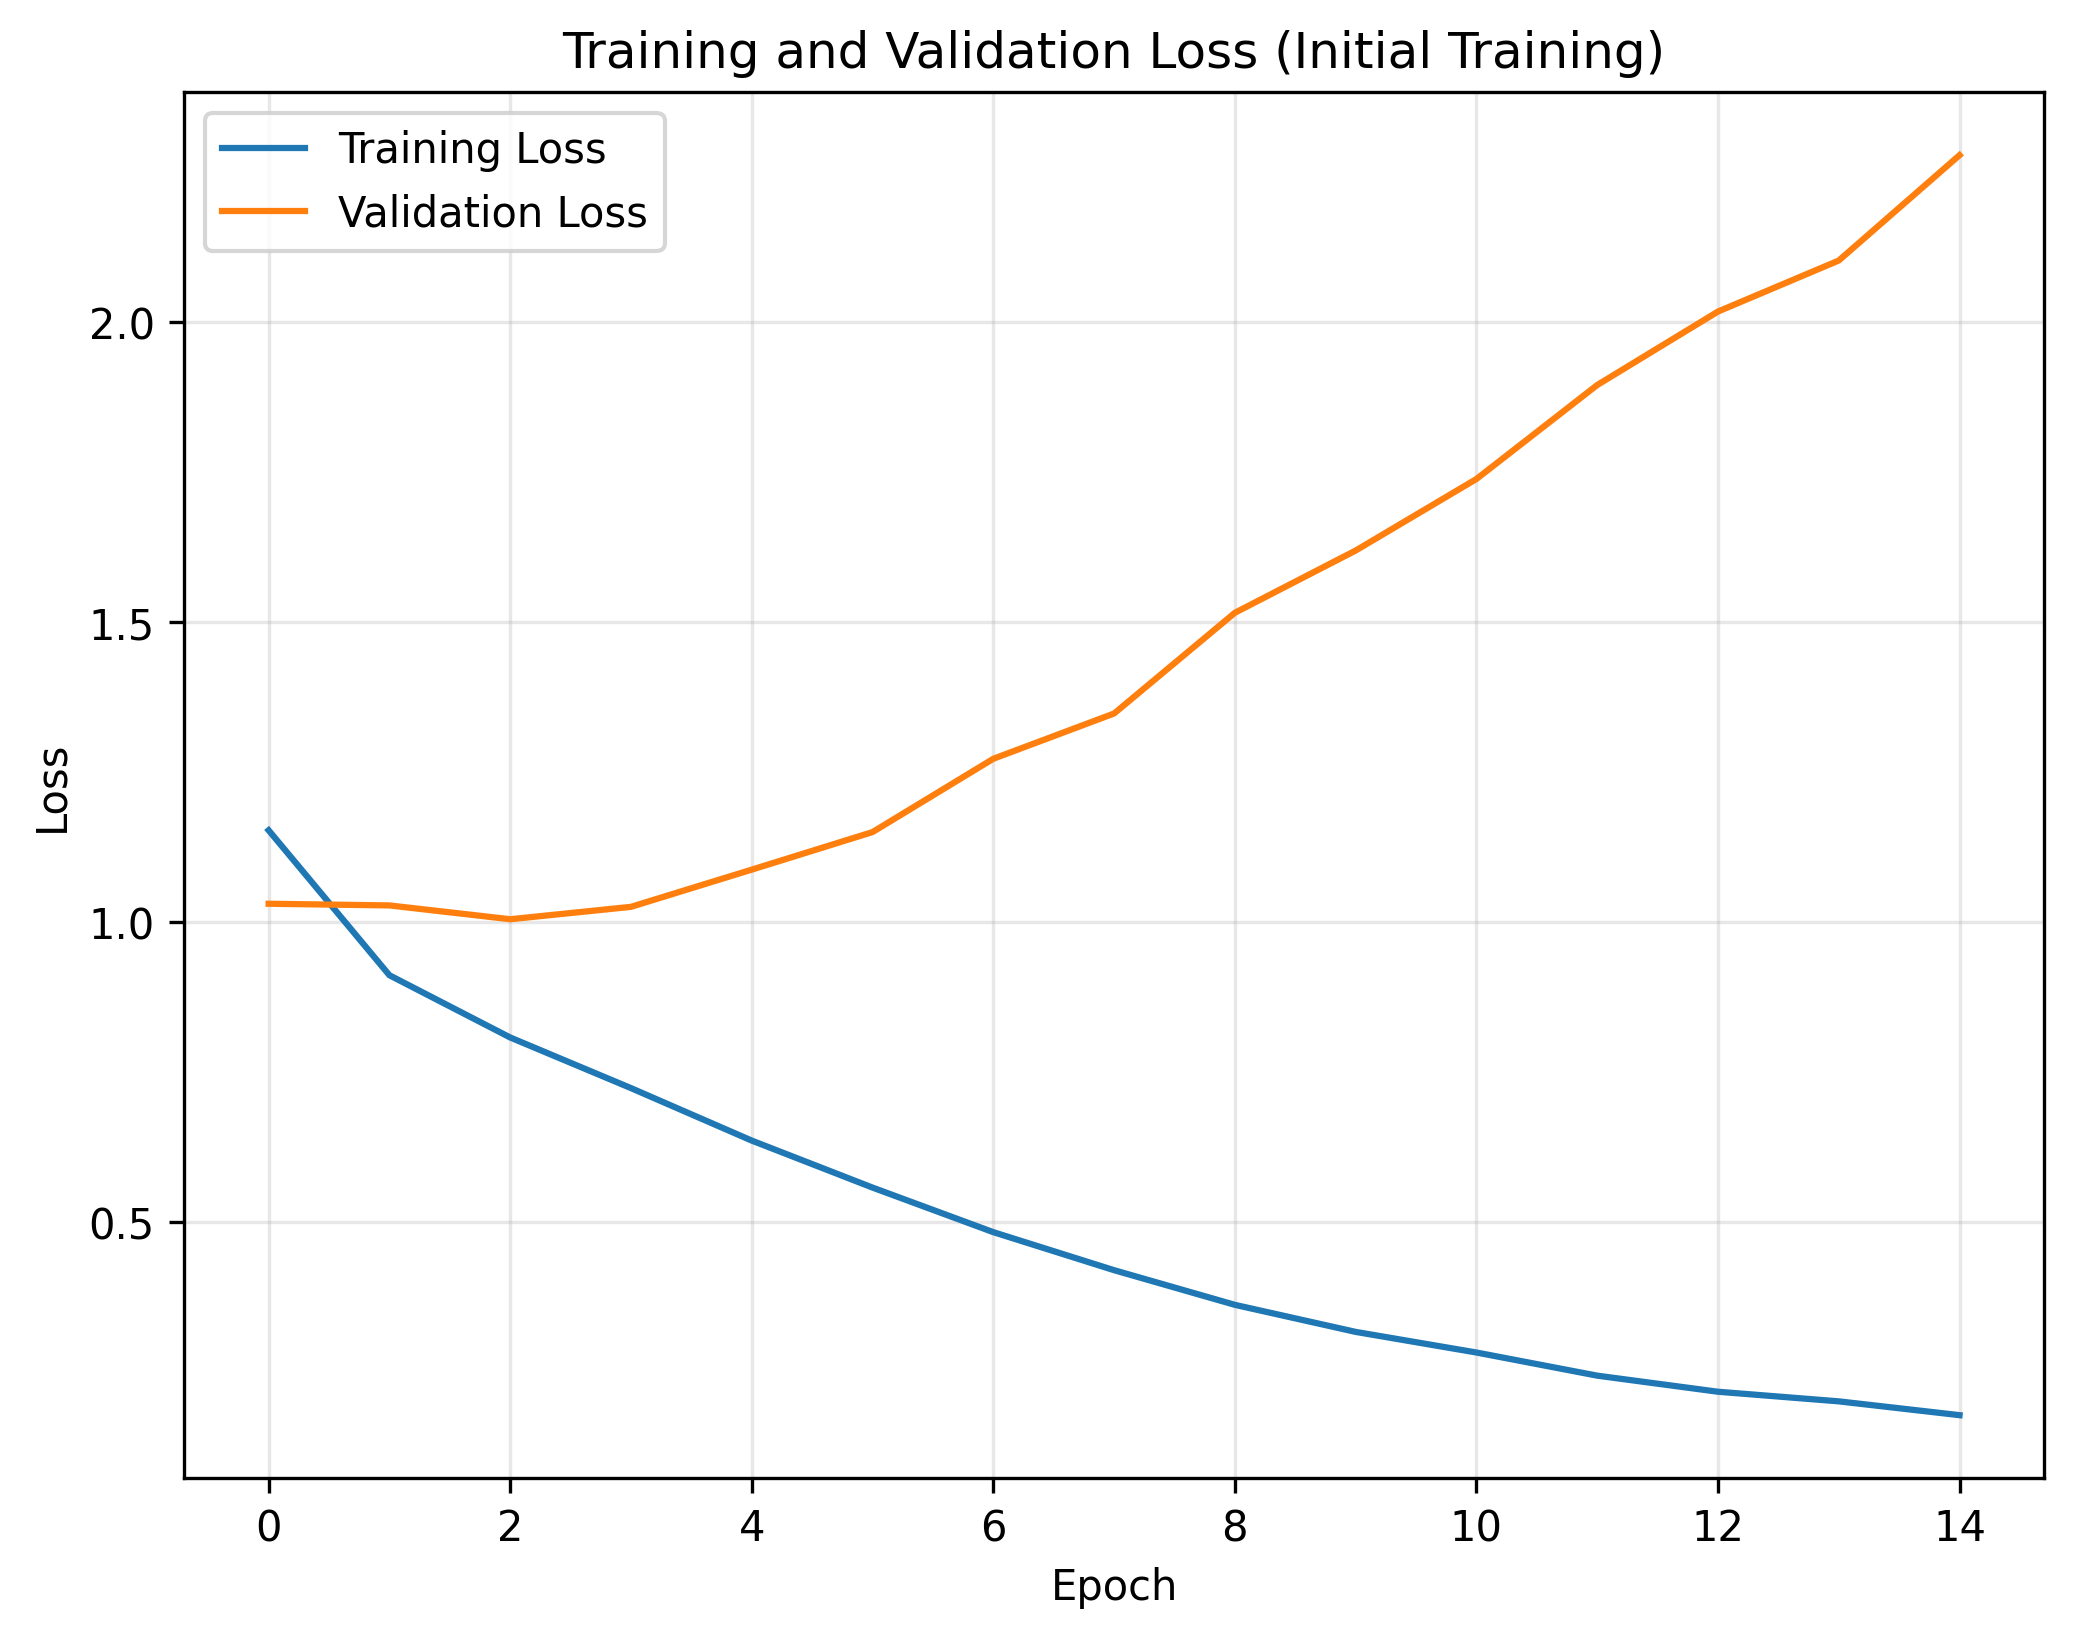
\includegraphics[width=0.7\textwidth]{plots/4_5_training_validation_loss.png}
\caption{Training vs Validation Loss -- ResNet50 (Initial Training, Frozen Base)}
\end{figure}

\noindent\textit{Inference:} Training loss decreased consistently from 1.15 to 0.18 across the 15 epochs, but validation loss increased steadily after epoch 3 (from about 1.00 to 2.28). This confirms the overfitting trend seen in the accuracy curves and motivates the fine-tuning stage.

\begin{figure}[H]
\centering
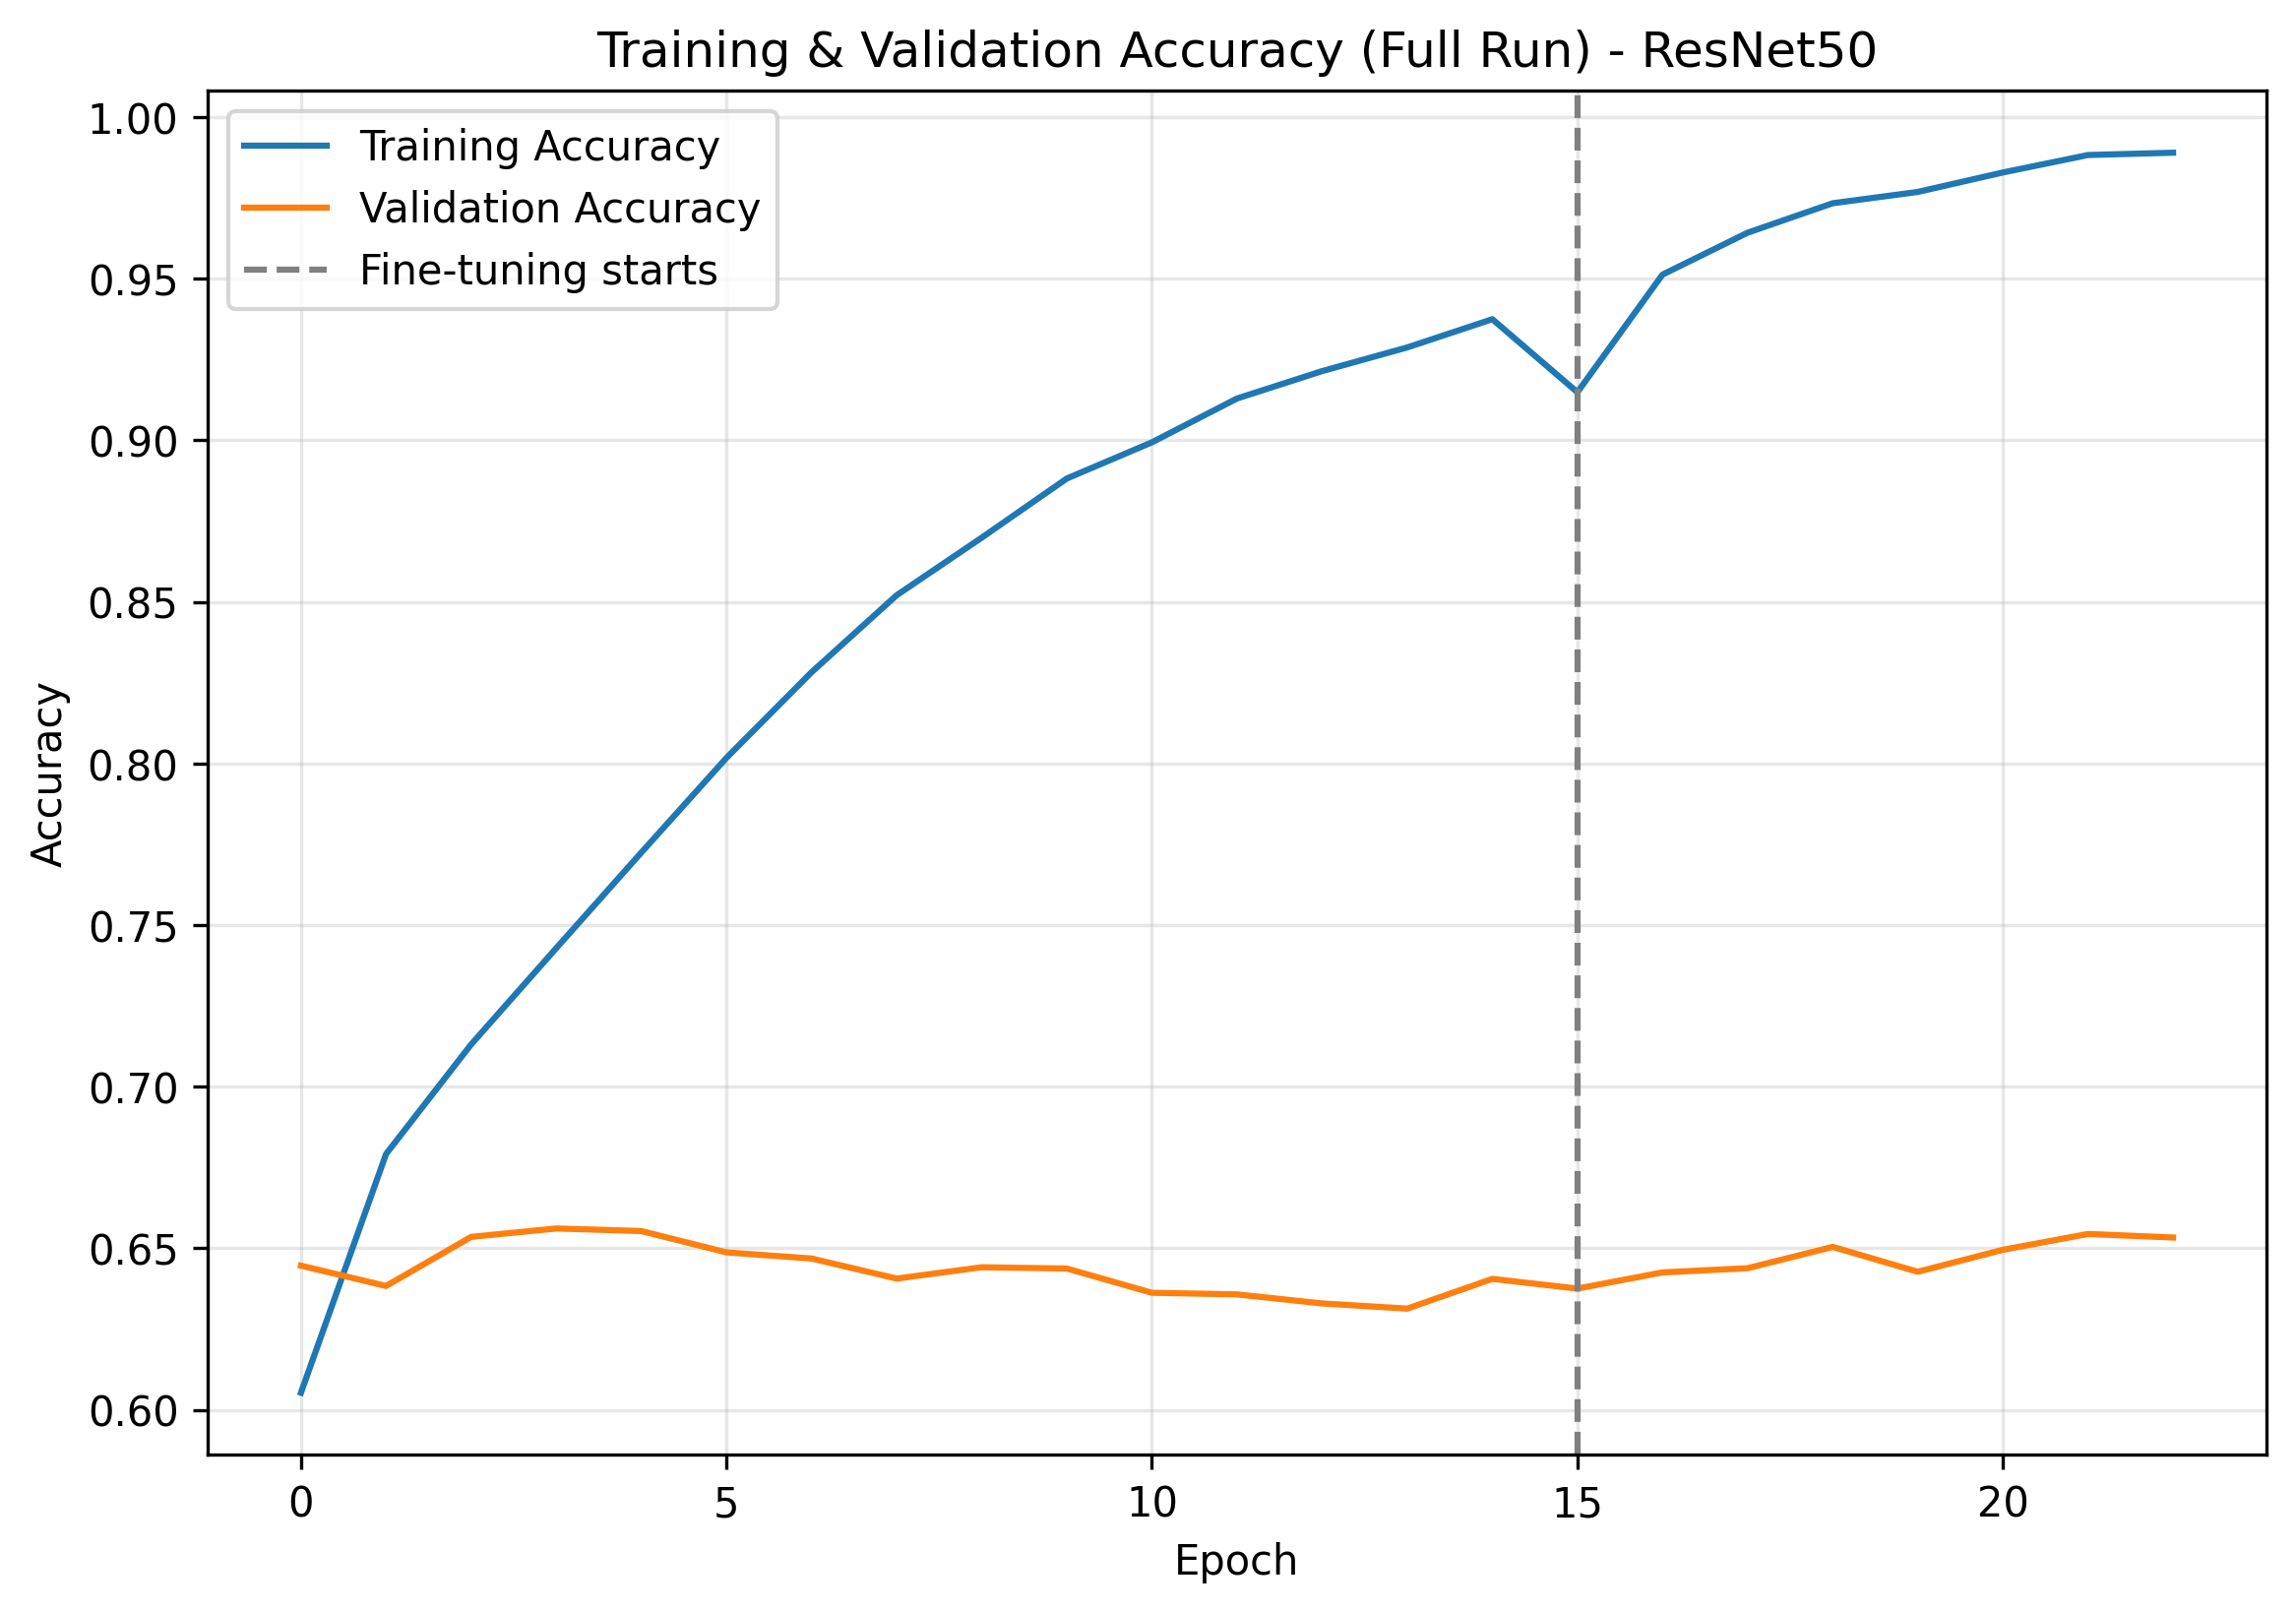
\includegraphics[width=0.7\textwidth]{plots/2b_combined_accuracy.png}
\caption{Combined Training and Validation Accuracy -- Initial Training + Fine-Tuning (ResNet50)}
\end{figure}

\noindent\textit{Inference:} The dashed line marks the start of fine-tuning. Validation accuracy improves from 64.05\% to a final 65.33\% once the last convolution block is unfrozen, while training accuracy climbs further to 98.90\%, showing the fine-tuned layers fit the training set more aggressively than they generalize.

\begin{figure}[H]
\centering
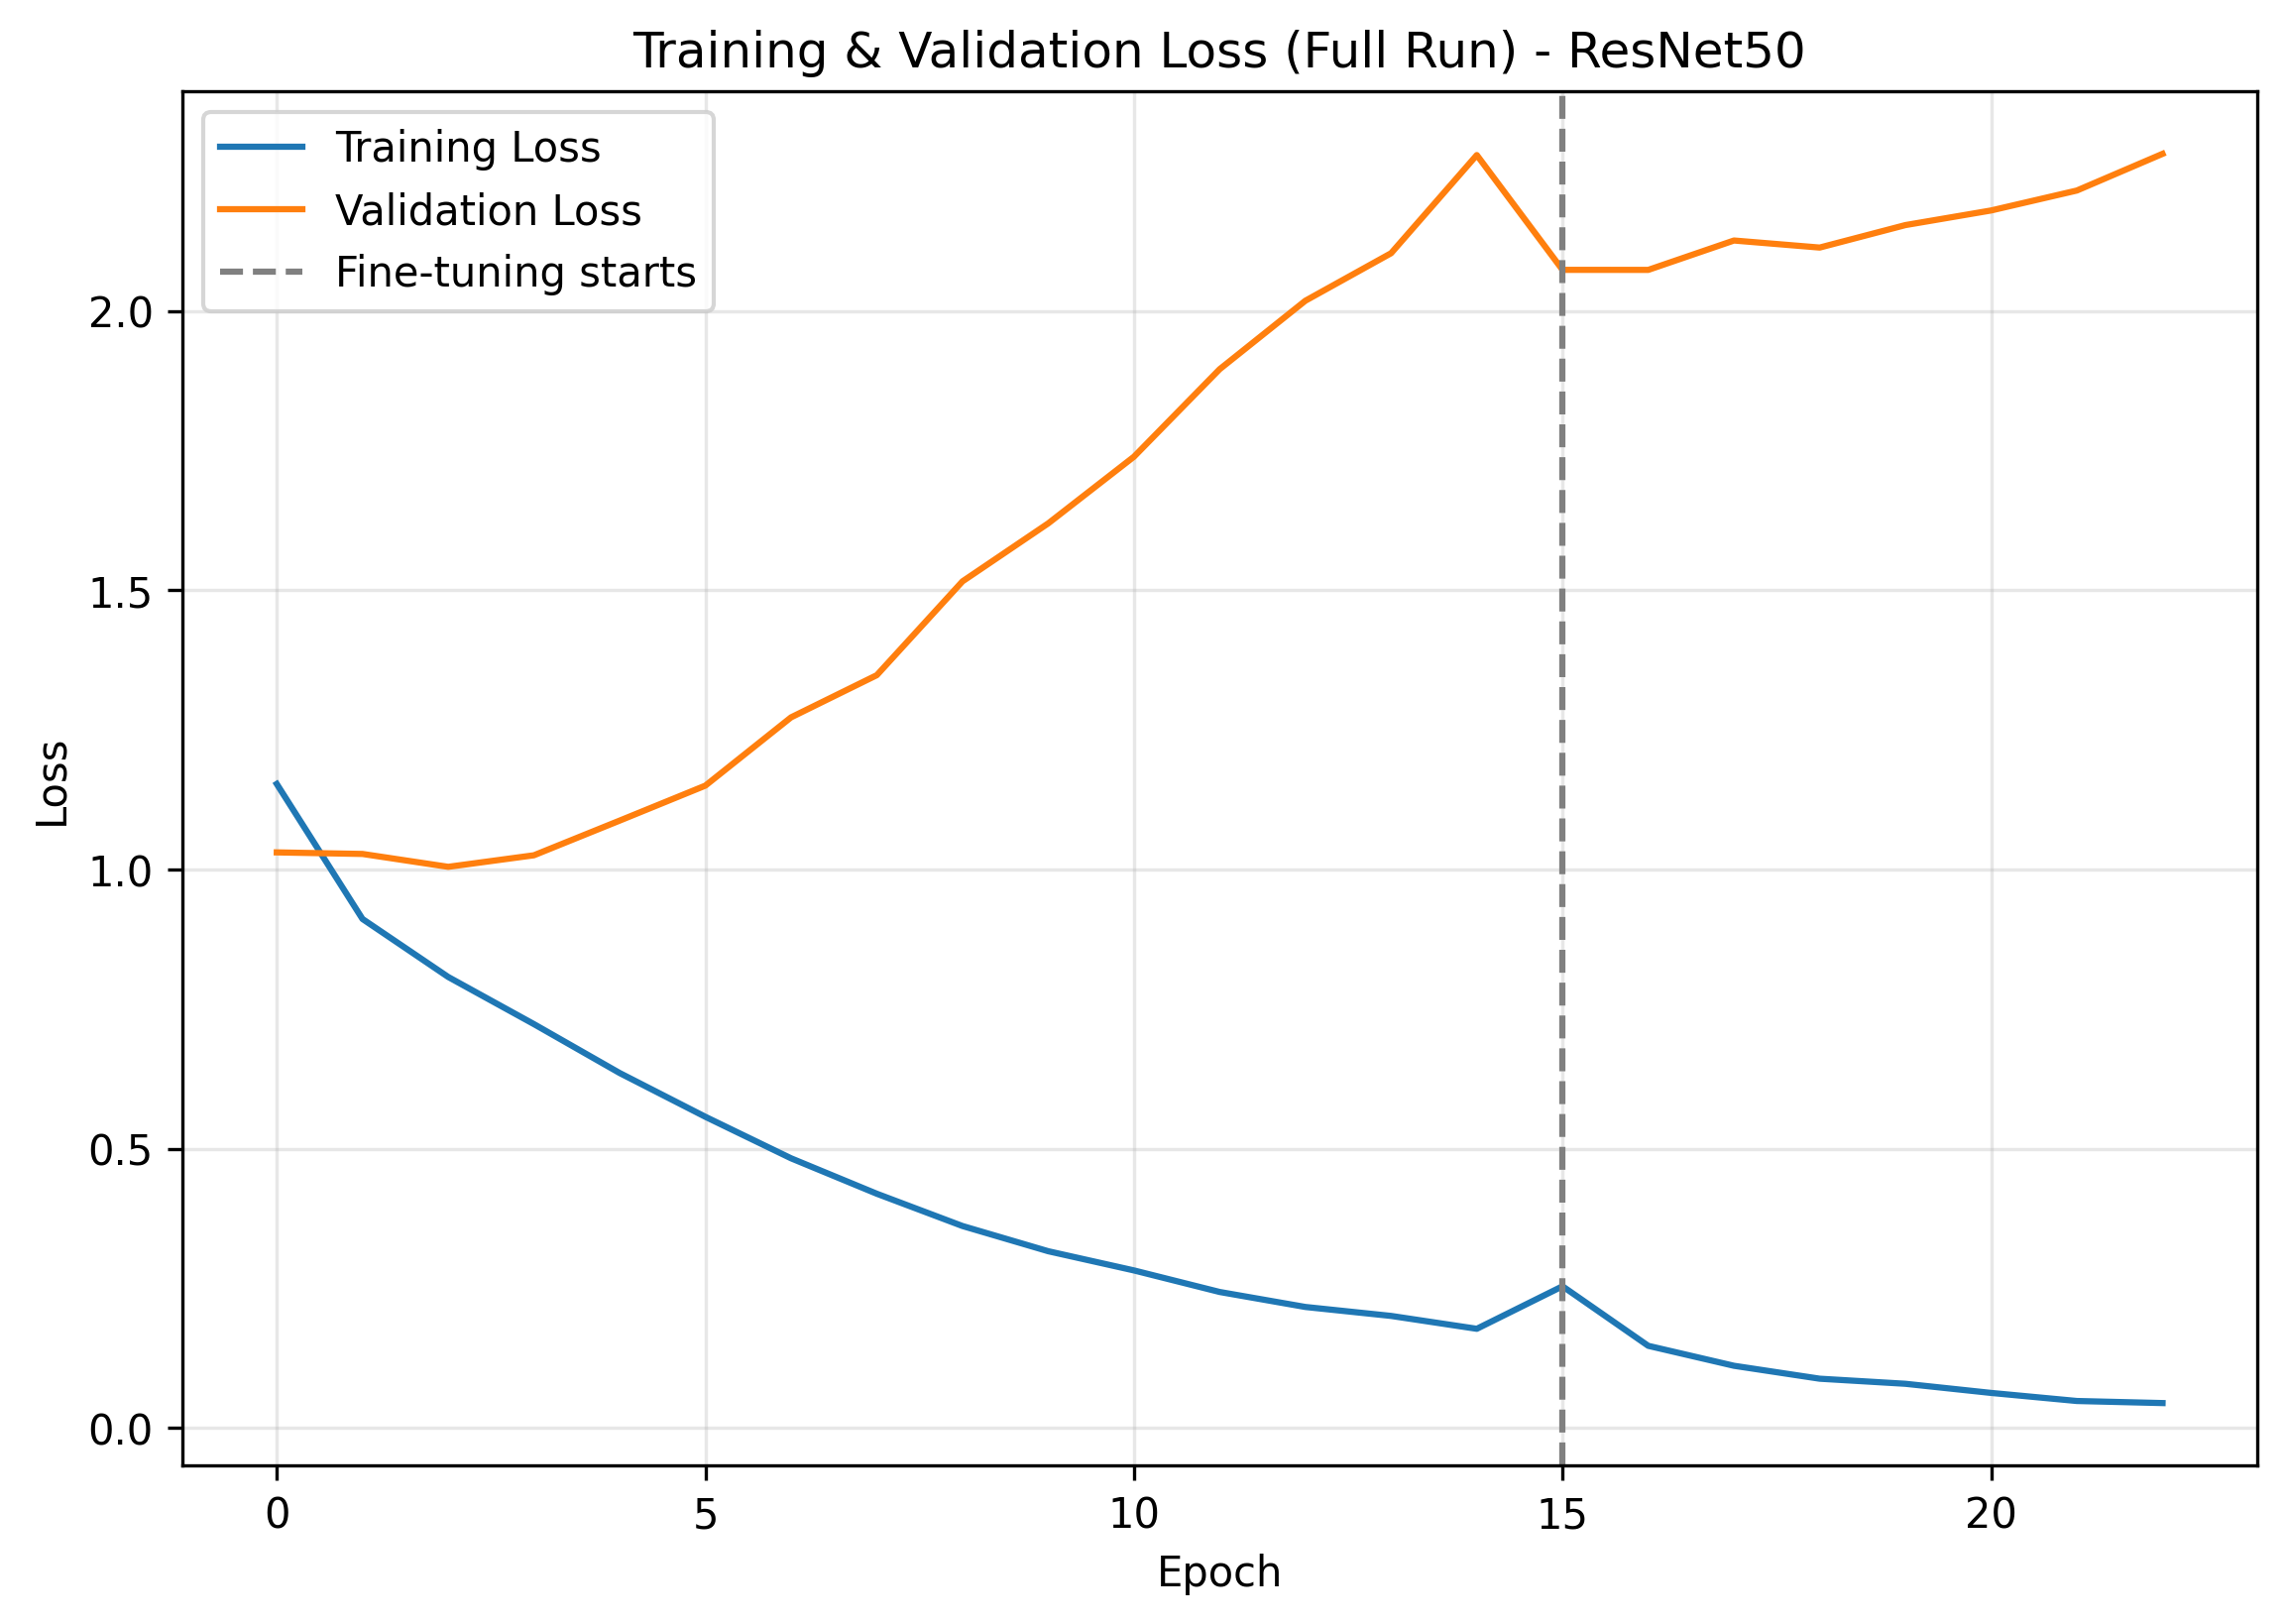
\includegraphics[width=0.7\textwidth]{plots/4b_combined_loss.png}
\caption{Combined Training and Validation Loss -- Initial Training + Fine-Tuning (ResNet50)}
\end{figure}

\noindent\textit{Inference:} Training loss continues to fall sharply during fine-tuning (down to 0.04), while validation loss keeps rising past the point where fine-tuning begins. This gap is the clearest evidence of overfitting once the deeper layers are unfrozen with a small CIFAR-10 image size.

\begin{figure}[H]
\centering
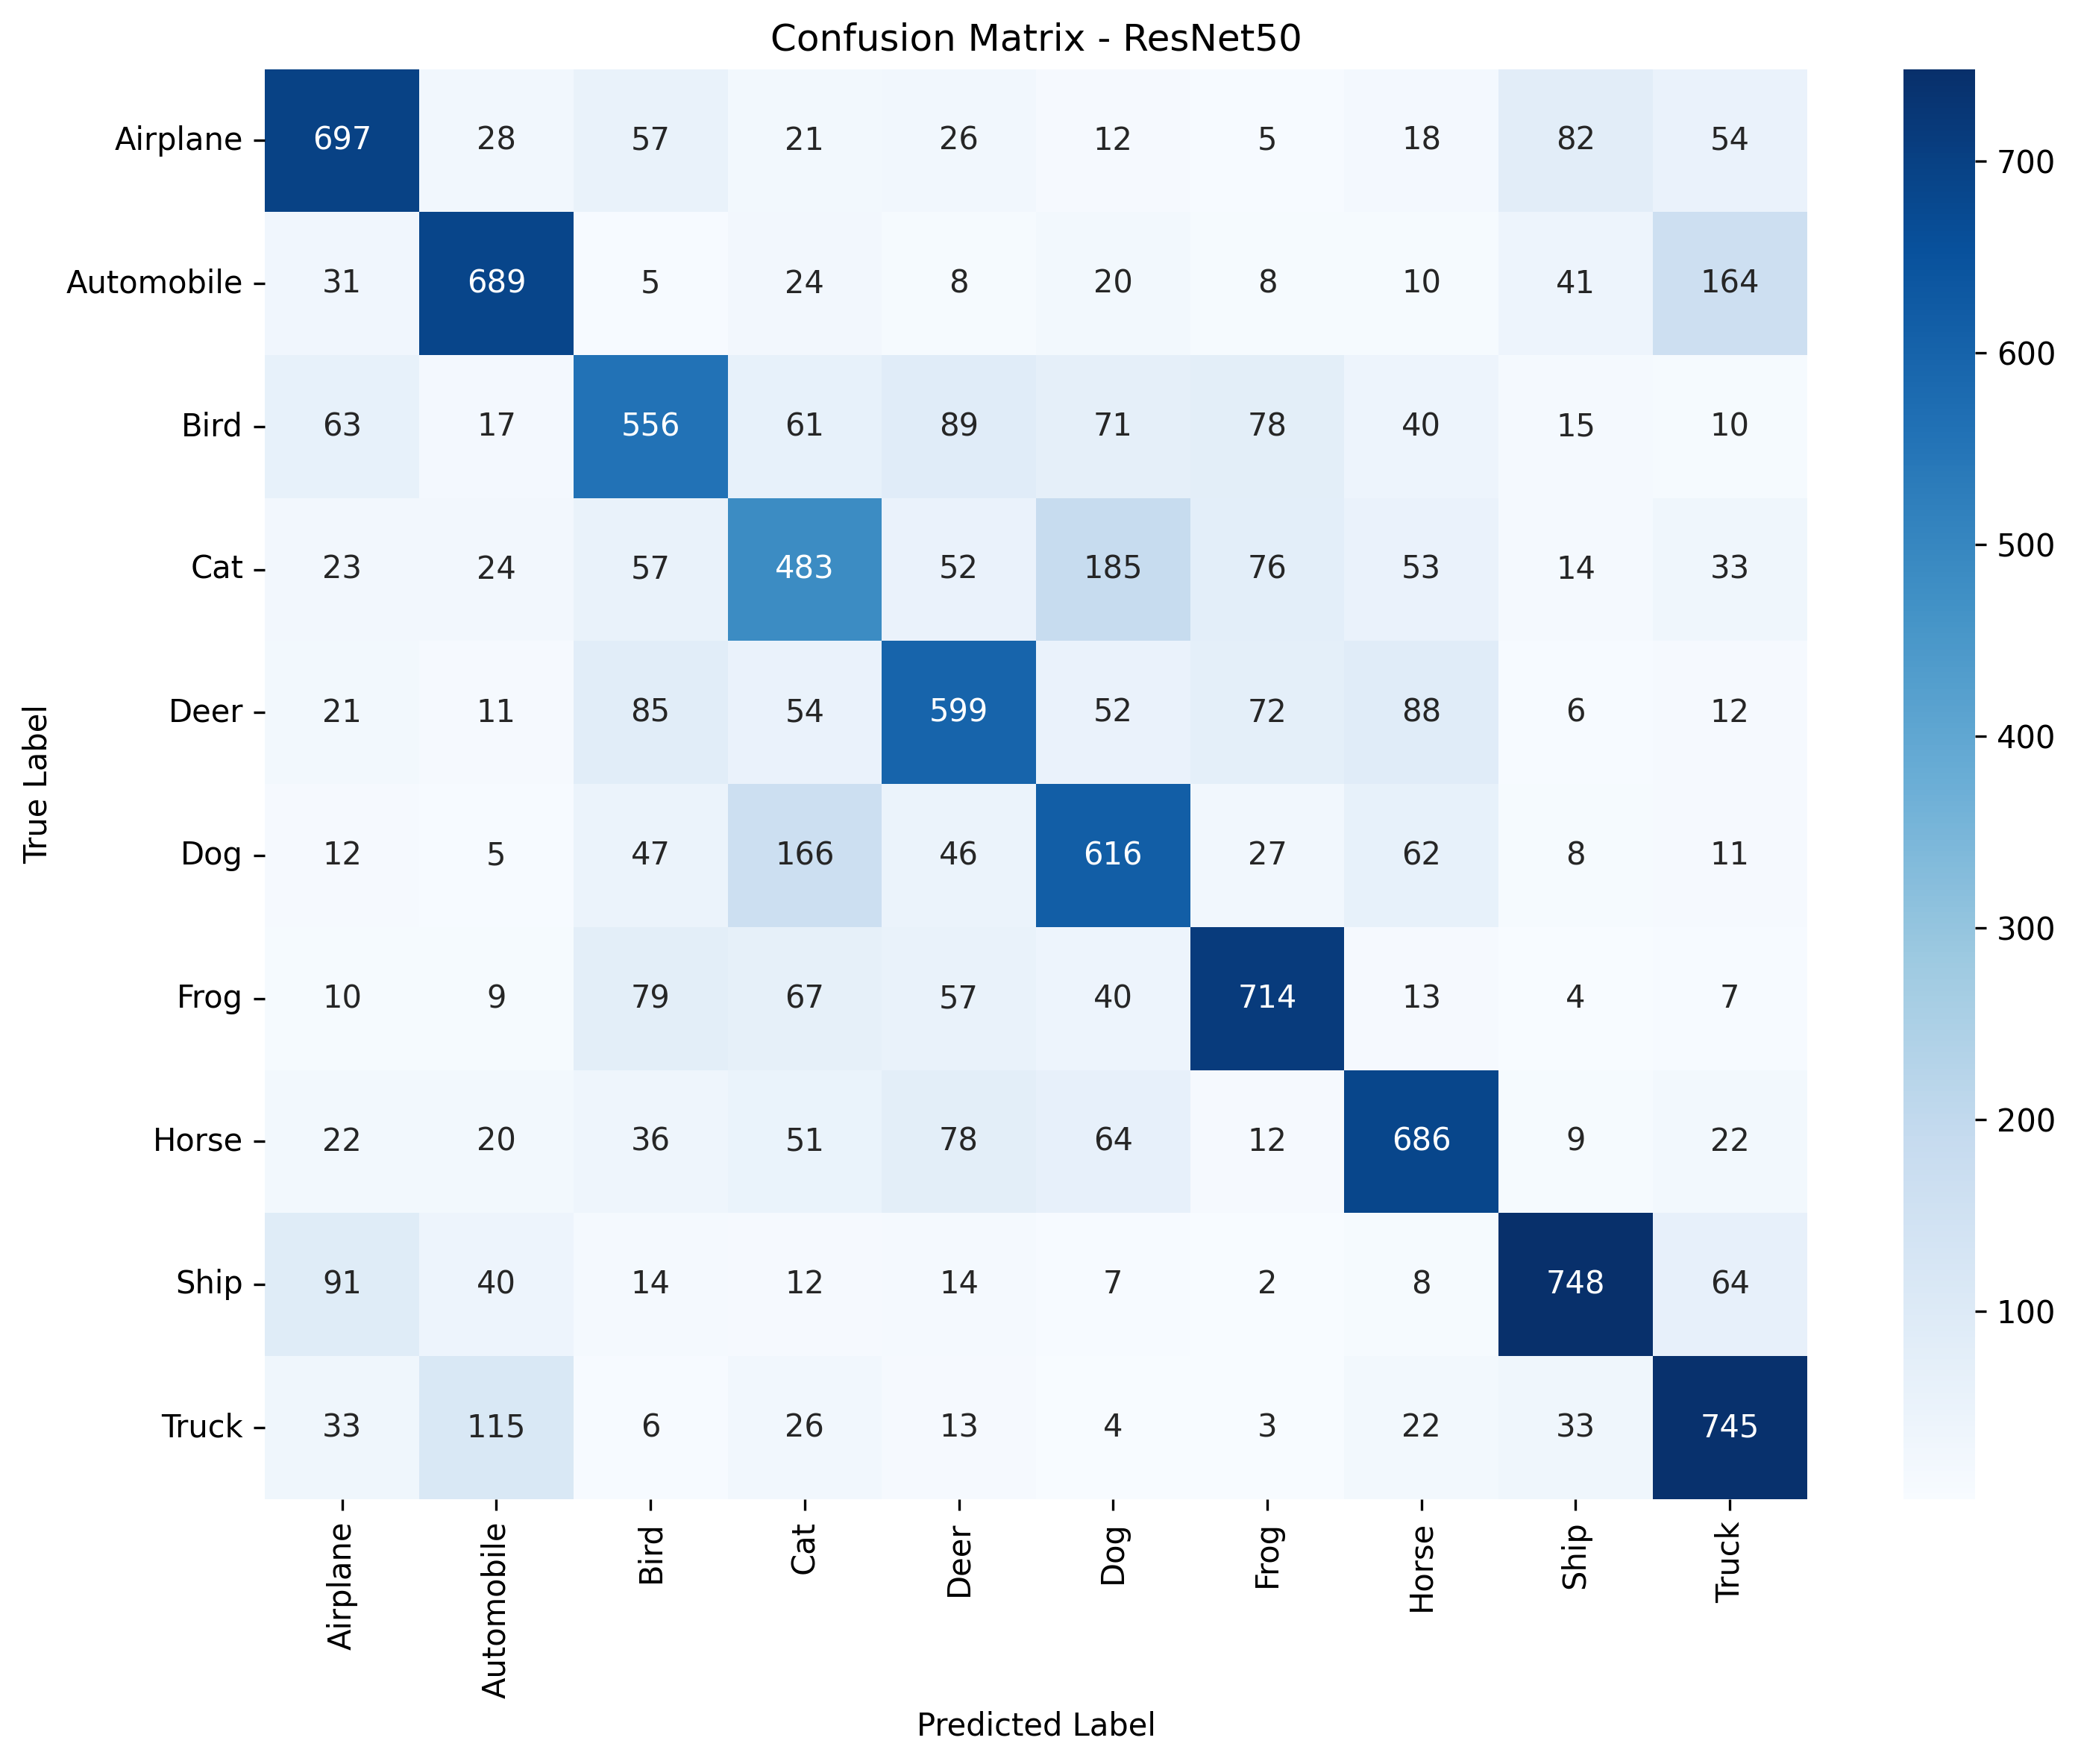
\includegraphics[width=0.7\textwidth]{plots/6_confusion_matrix.png}
\caption{Confusion Matrix -- ResNet50}
\end{figure}

\noindent\textit{Inference:} ResNet50 performs best on the Ship (76\% F1) and Frog (72\% F1) classes, while Cat (49\% F1) and Bird (57\% F1) show the most confusion, frequently being mistaken for visually similar animal classes such as Dog and Deer.

\begin{figure}[H]
\centering
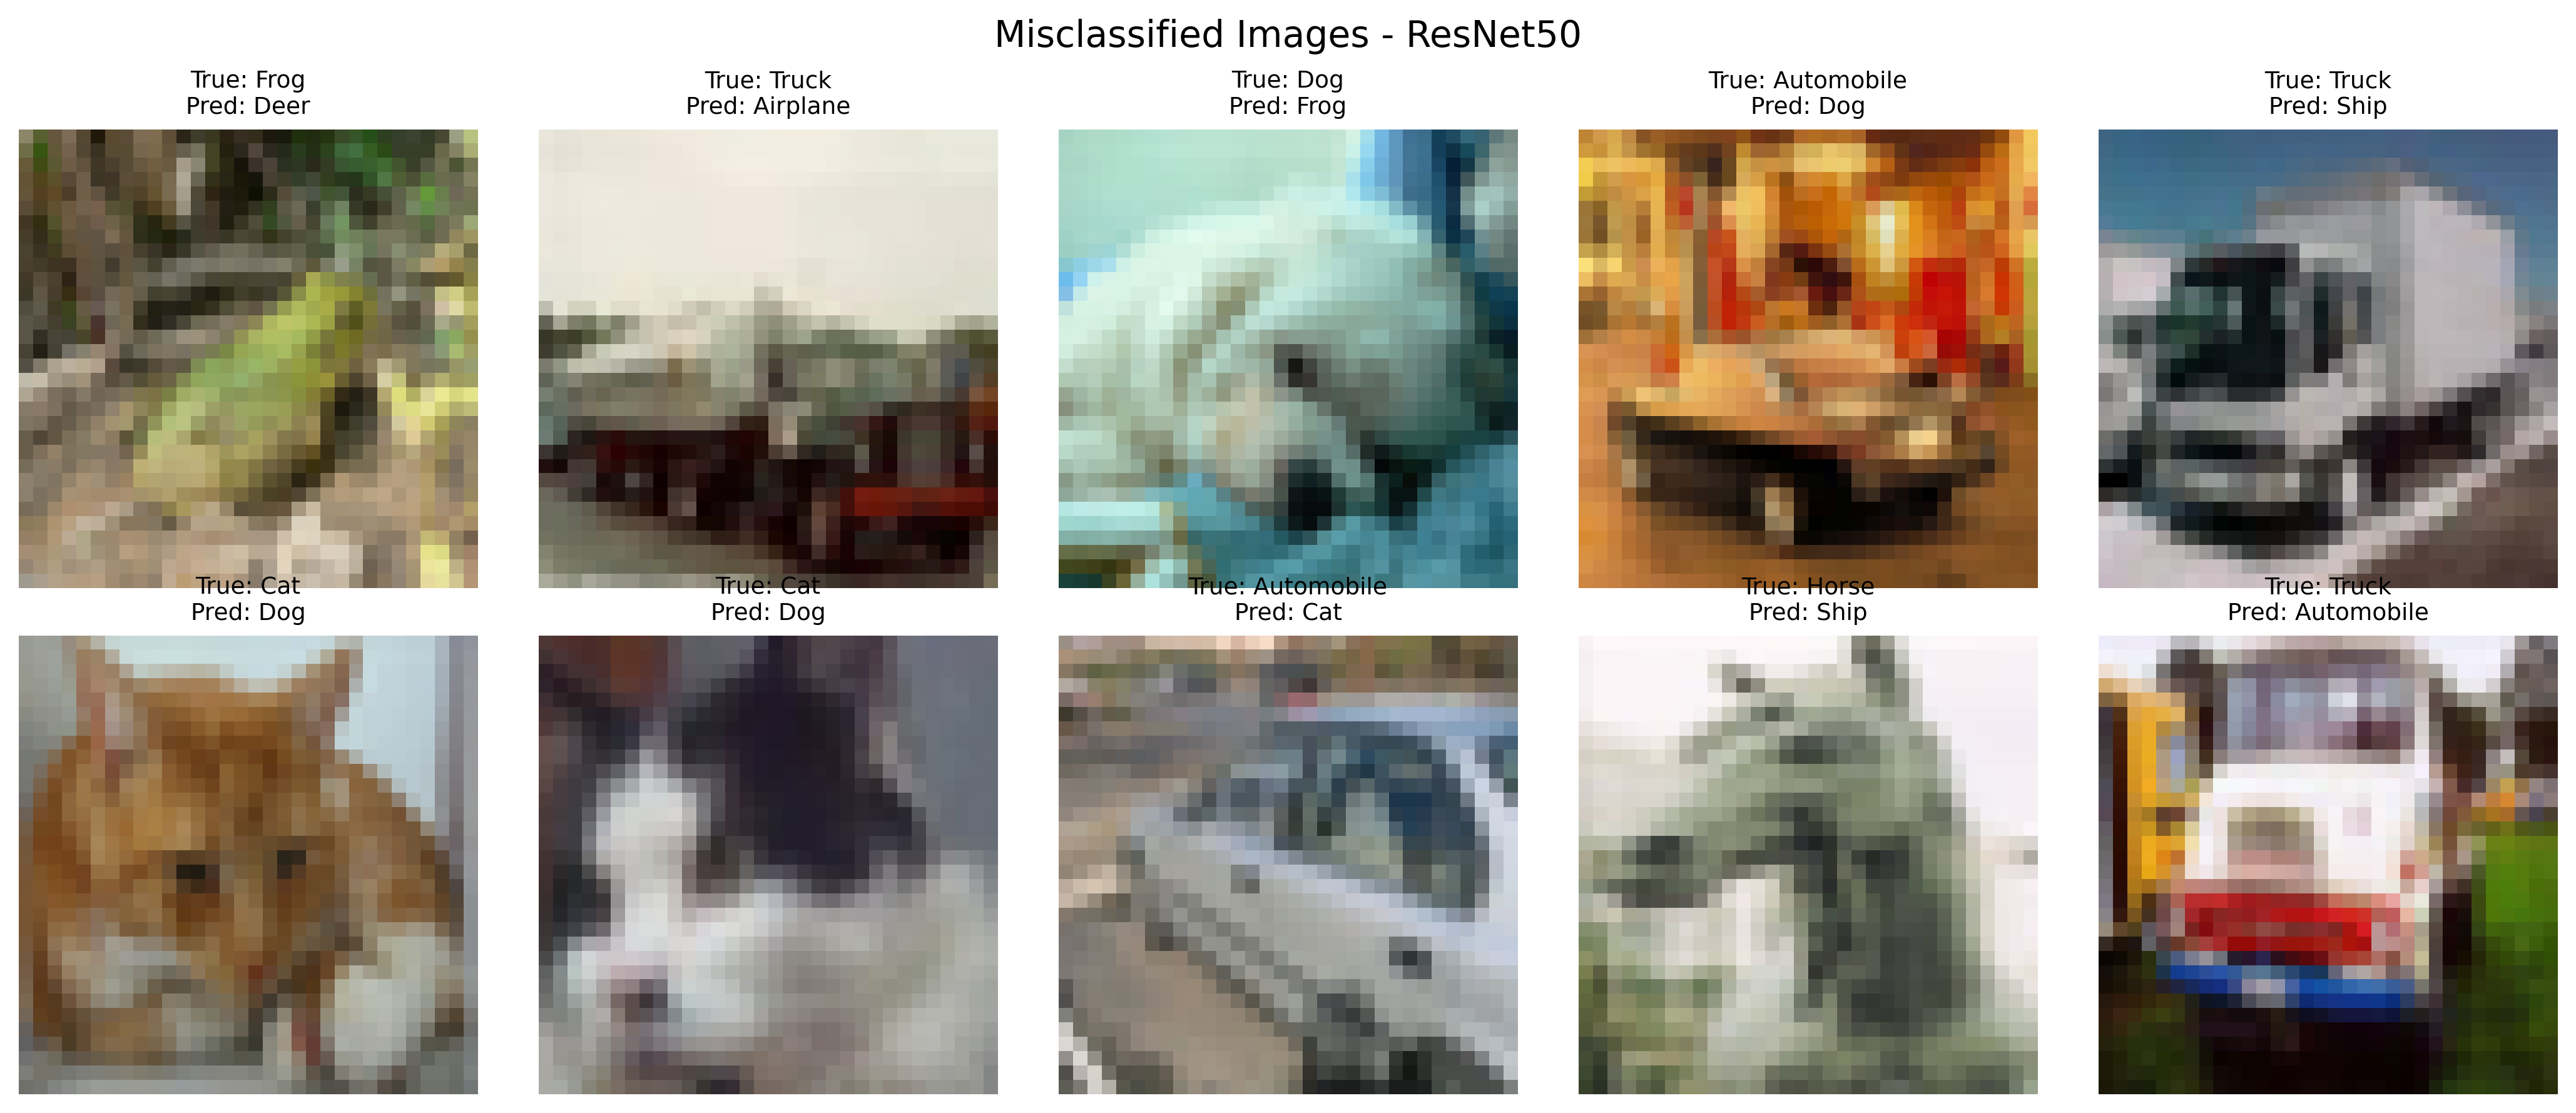
\includegraphics[width=0.75\textwidth]{plots/7_misclassified_images.png}
\caption{Misclassified Images -- ResNet50 (Optional)}
\end{figure}

\noindent\textit{Inference:} 3,467 of the 10,000 test images (34.67\%) were misclassified by ResNet50. The sampled misclassifications mostly occur between visually or semantically close categories (e.g., cat/dog, automobile/truck), consistent with the per-class precision and recall values in the classification report.

\begin{figure}[H]
\centering
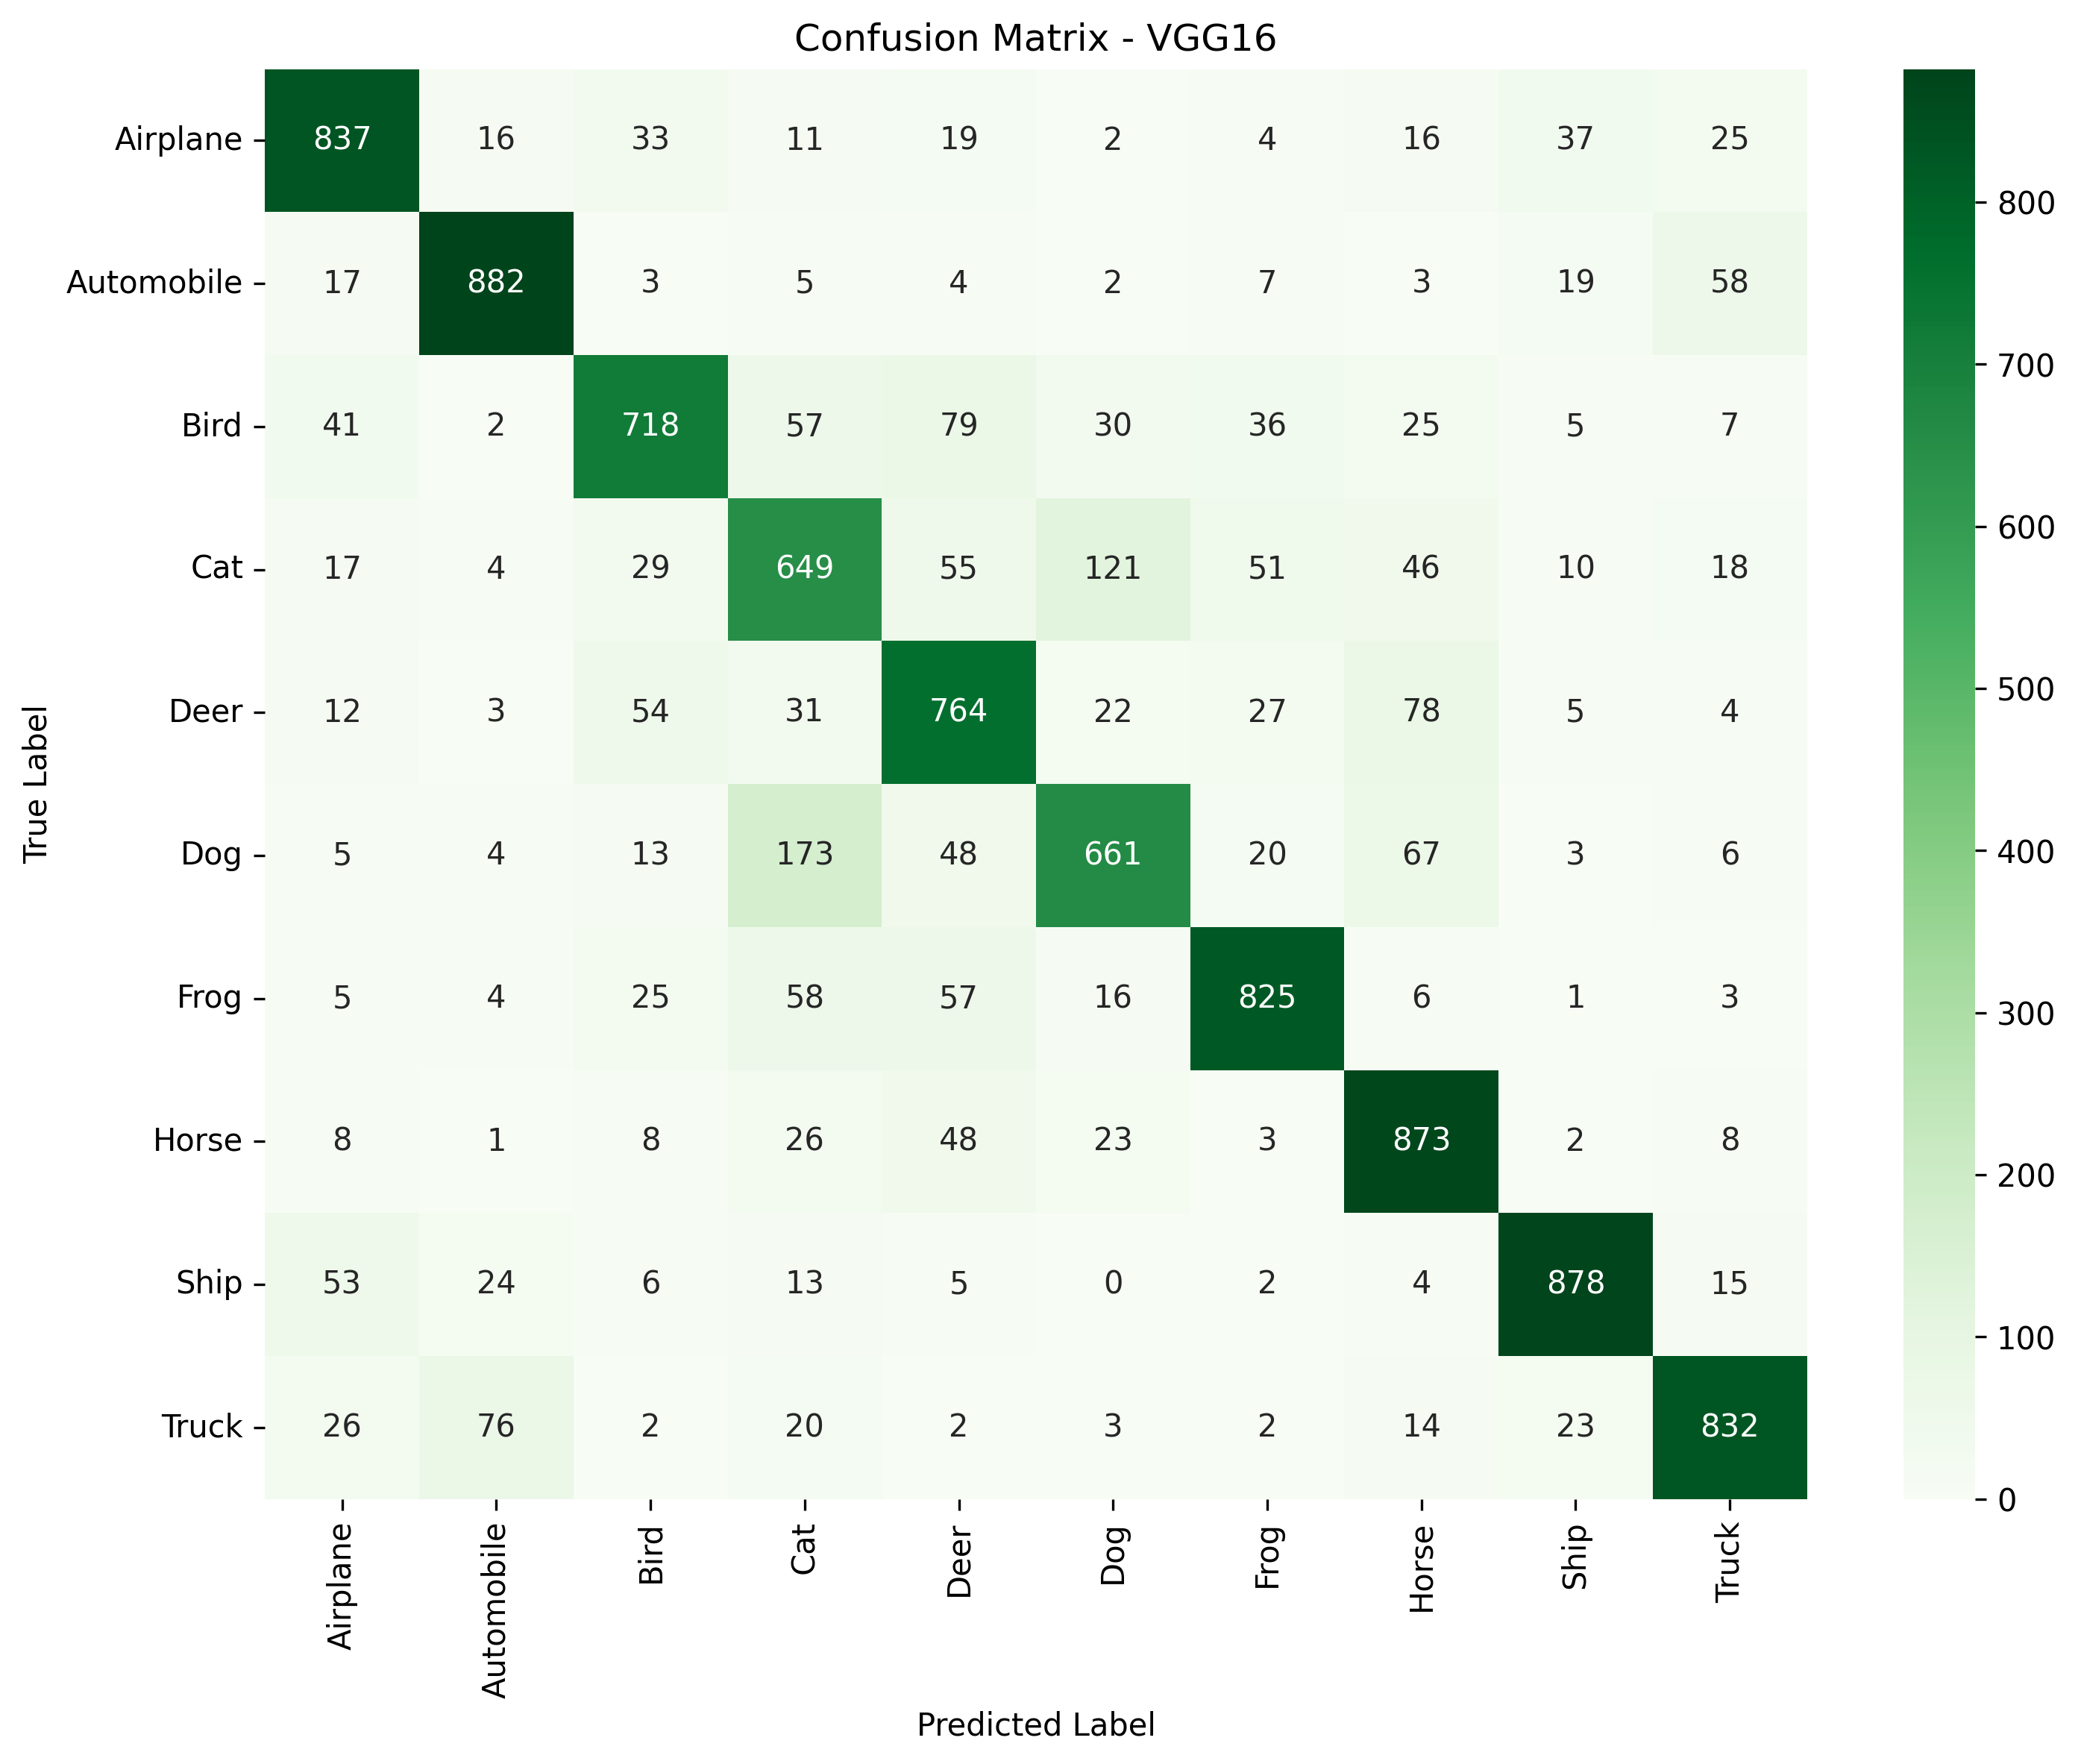
\includegraphics[width=0.7\textwidth]{plots/6b_confusion_matrix_vgg16.png}
\caption{Confusion Matrix -- VGG16}
\end{figure}

\noindent\textit{Inference:} VGG16 reaches 79.19\% test accuracy with more balanced per-class performance than ResNet50, benefiting from full fine-tuning of its deep $3\times3$ filter stack even at the small $32\times32$ input size.

\begin{figure}[H]
\centering
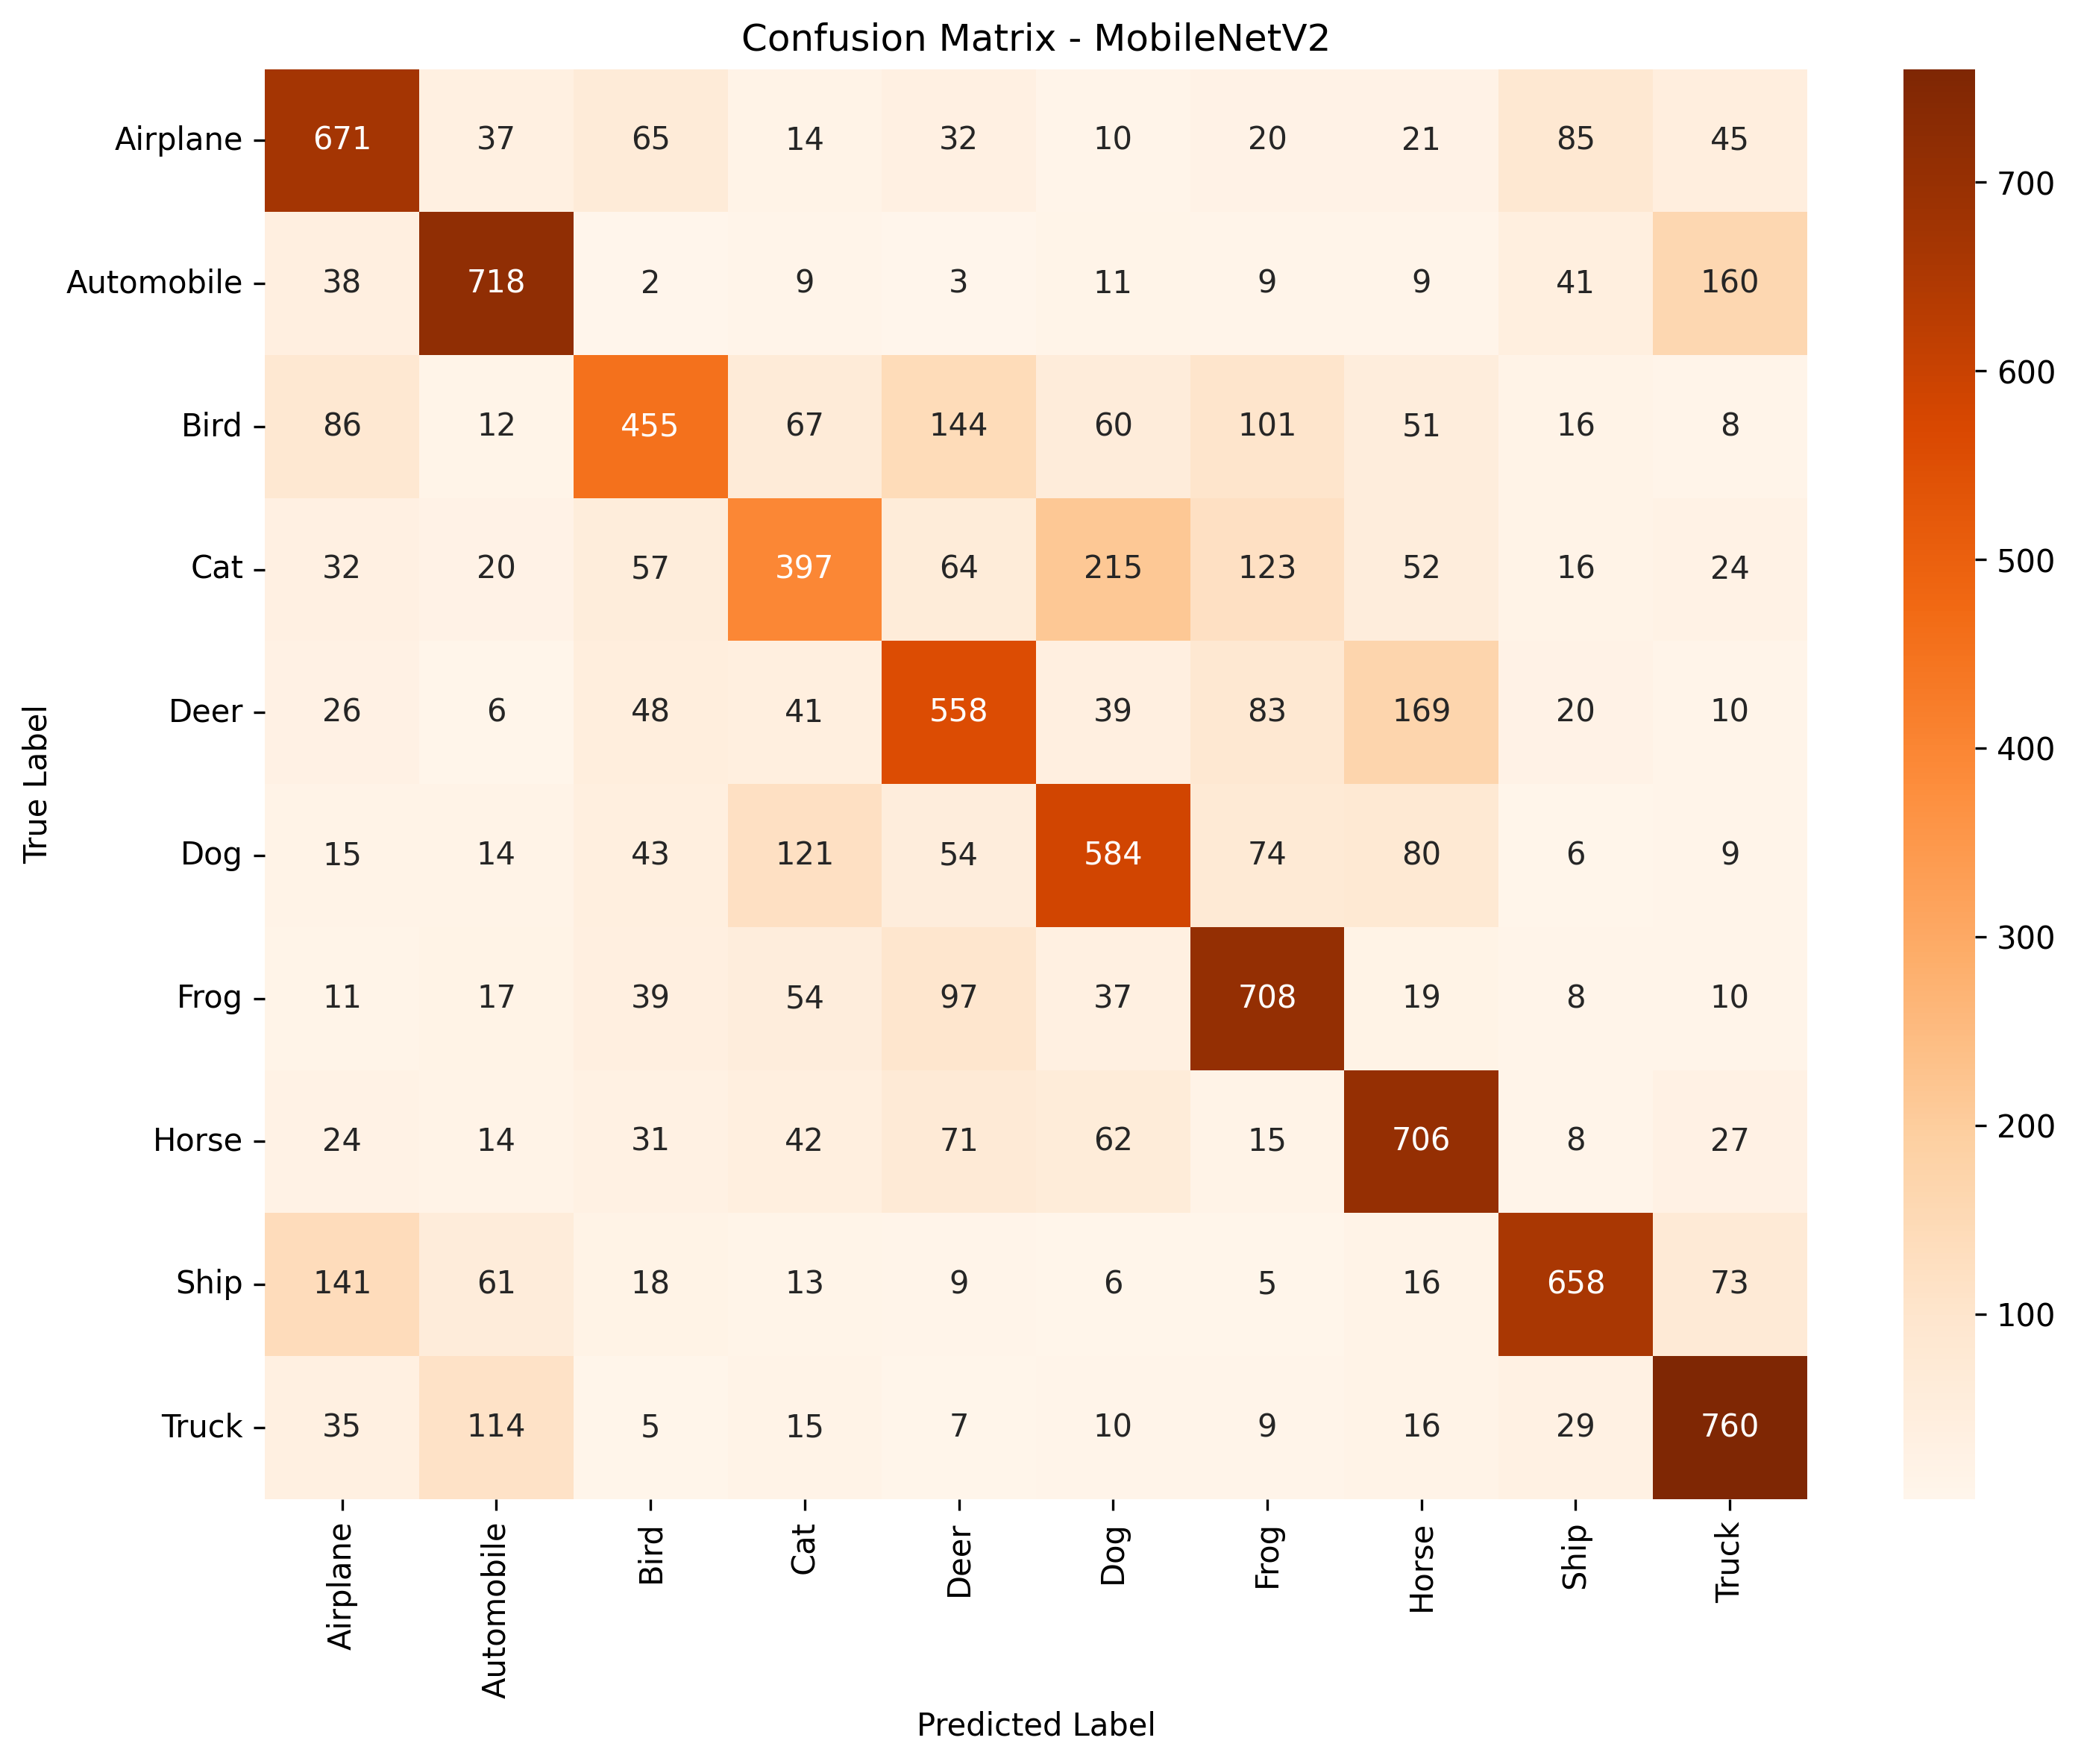
\includegraphics[width=0.7\textwidth]{plots/6c_confusion_matrix_mobilenetv2.png}
\caption{Confusion Matrix -- MobileNetV2}
\end{figure}

\noindent\textit{Inference:} MobileNetV2 shows the weakest performance among the transfer-learning models at 62.15\% accuracy. Its lightweight depthwise-separable design, pretrained at $224\times224$, adapts less effectively to the very small $32\times32$ CIFAR-10 input than the larger ResNet50 and VGG16 backbones.

\begin{figure}[H]
\centering
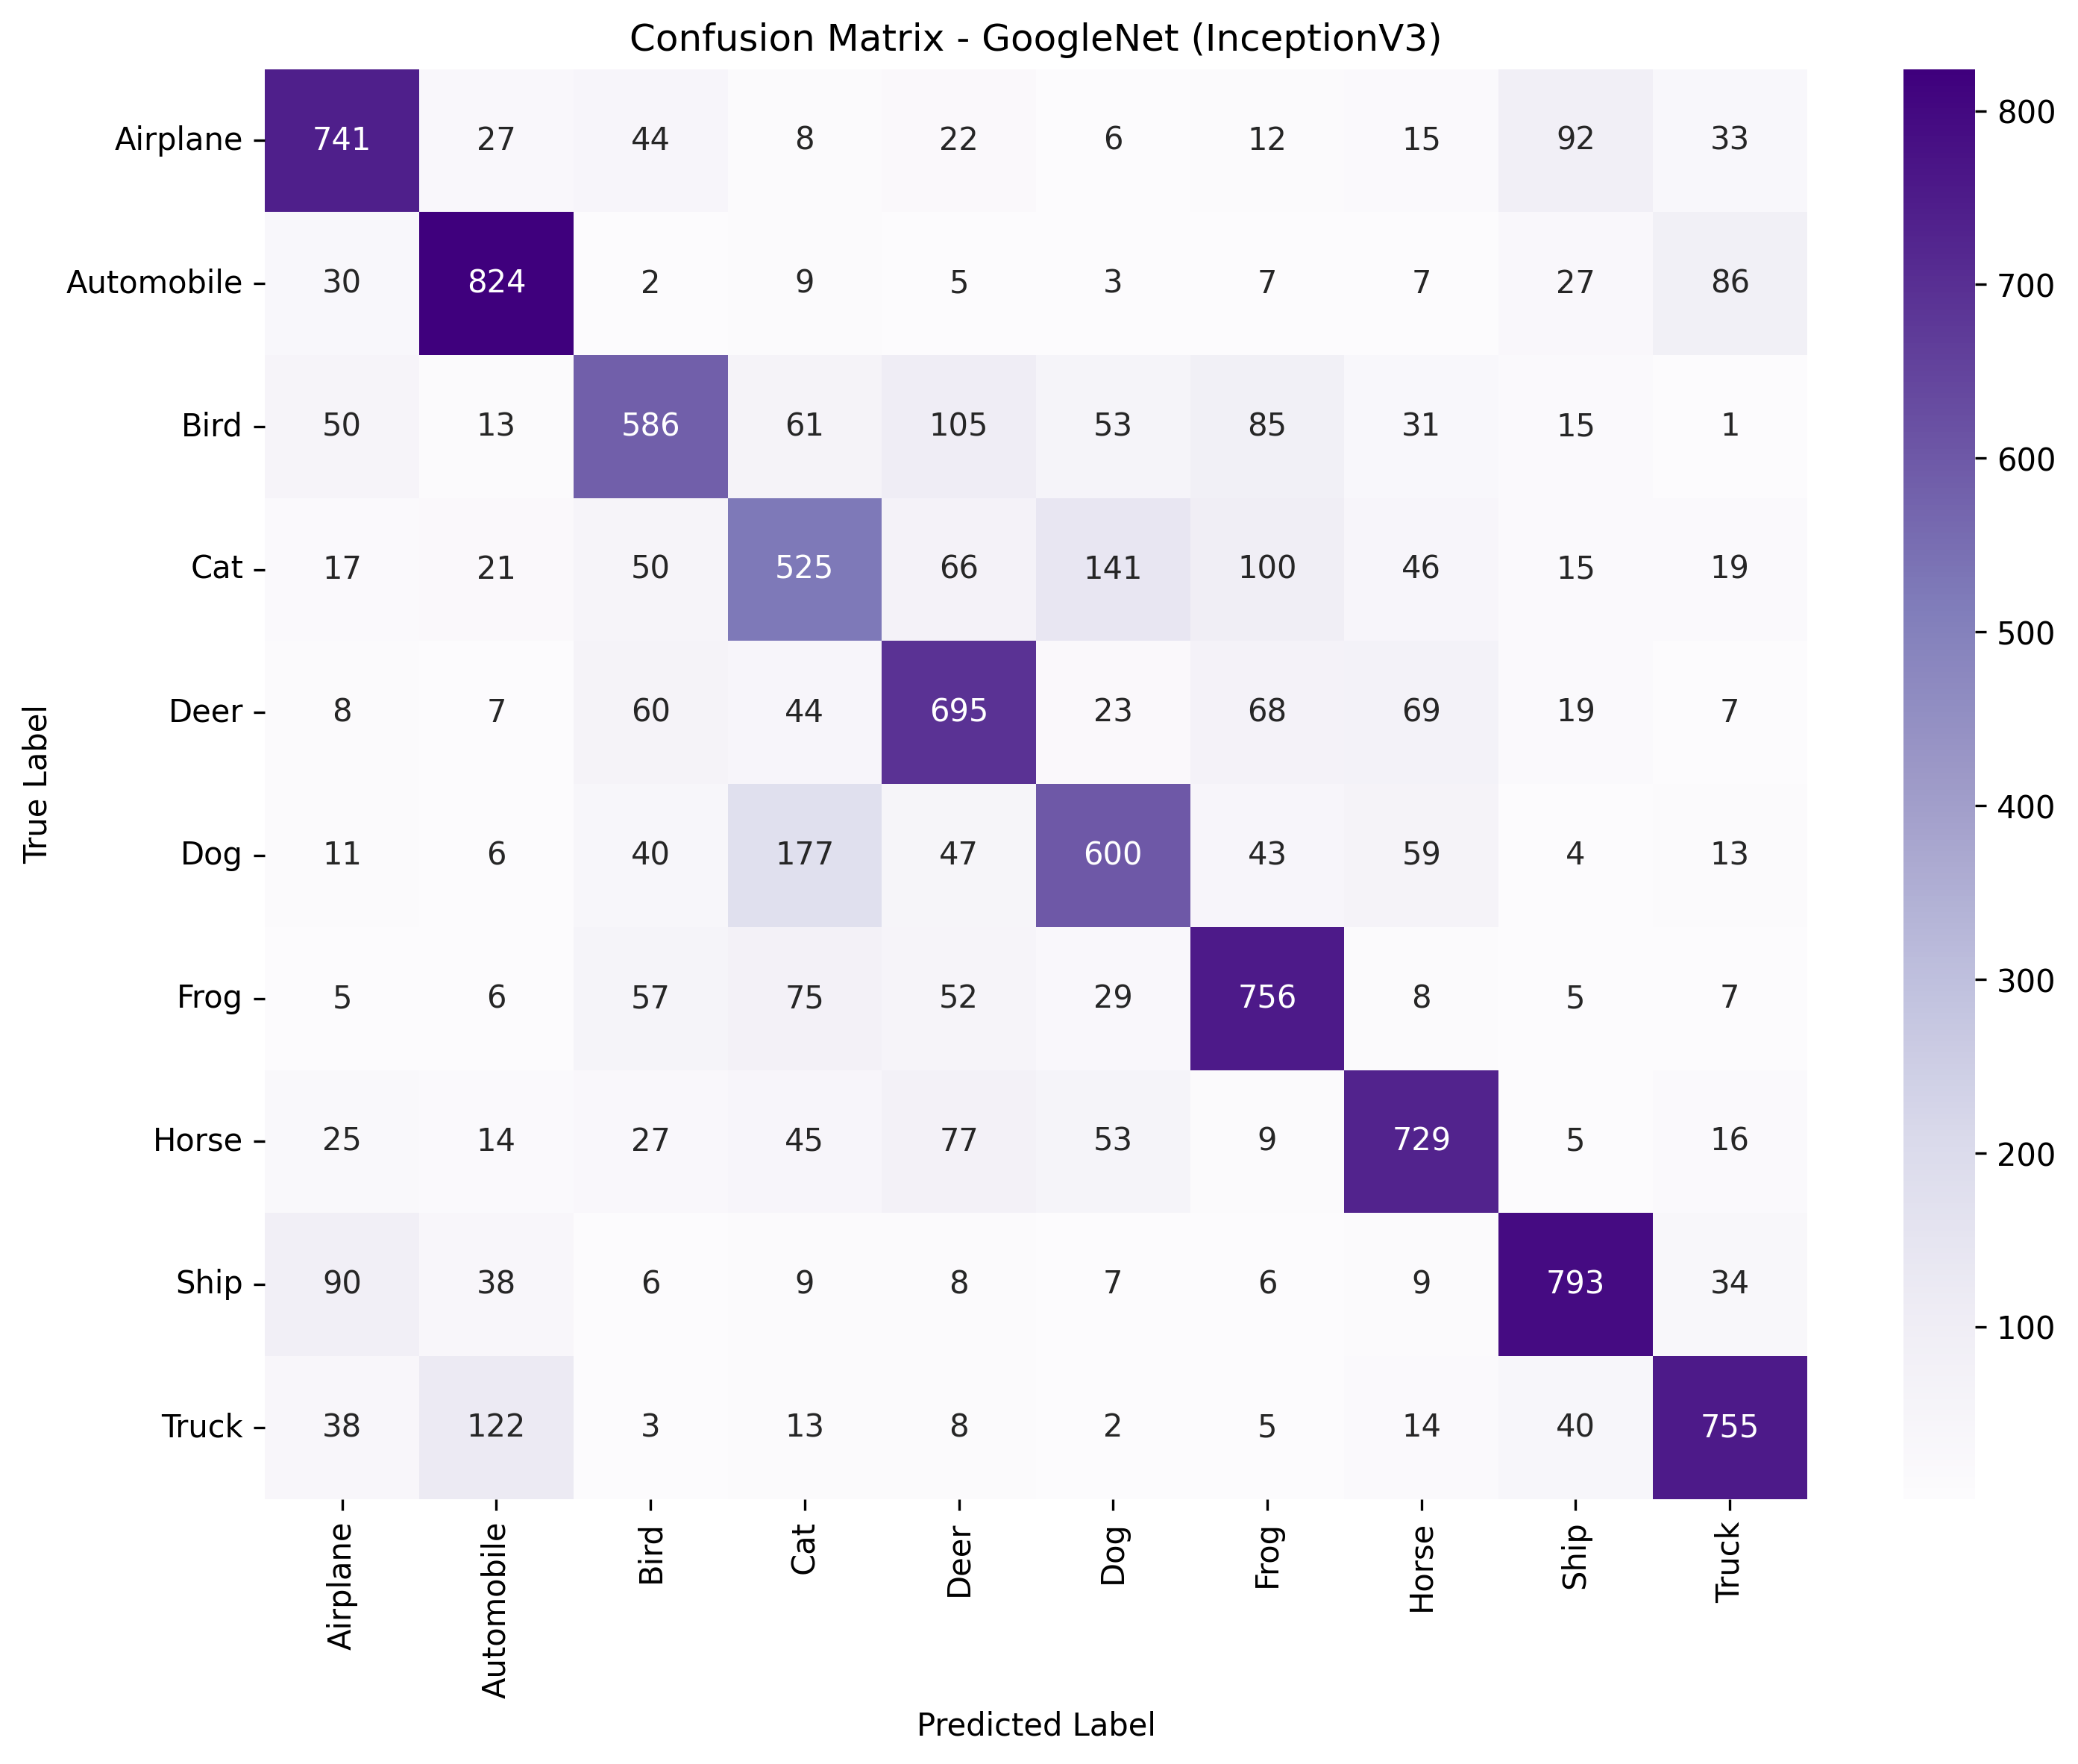
\includegraphics[width=0.7\textwidth]{plots/6d_confusion_matrix_googlenet.png}
\caption{Confusion Matrix -- GoogleNet (InceptionV3)}
\end{figure}

\noindent\textit{Inference:} InceptionV3, evaluated after resizing CIFAR-10 images to $75\times75$, reaches 70.04\% test accuracy. Its multi-scale Inception filters help, but up-sampling from a $32\times32$ source introduces interpolation artifacts that likely limit further gains.

\begin{figure}[H]
\centering
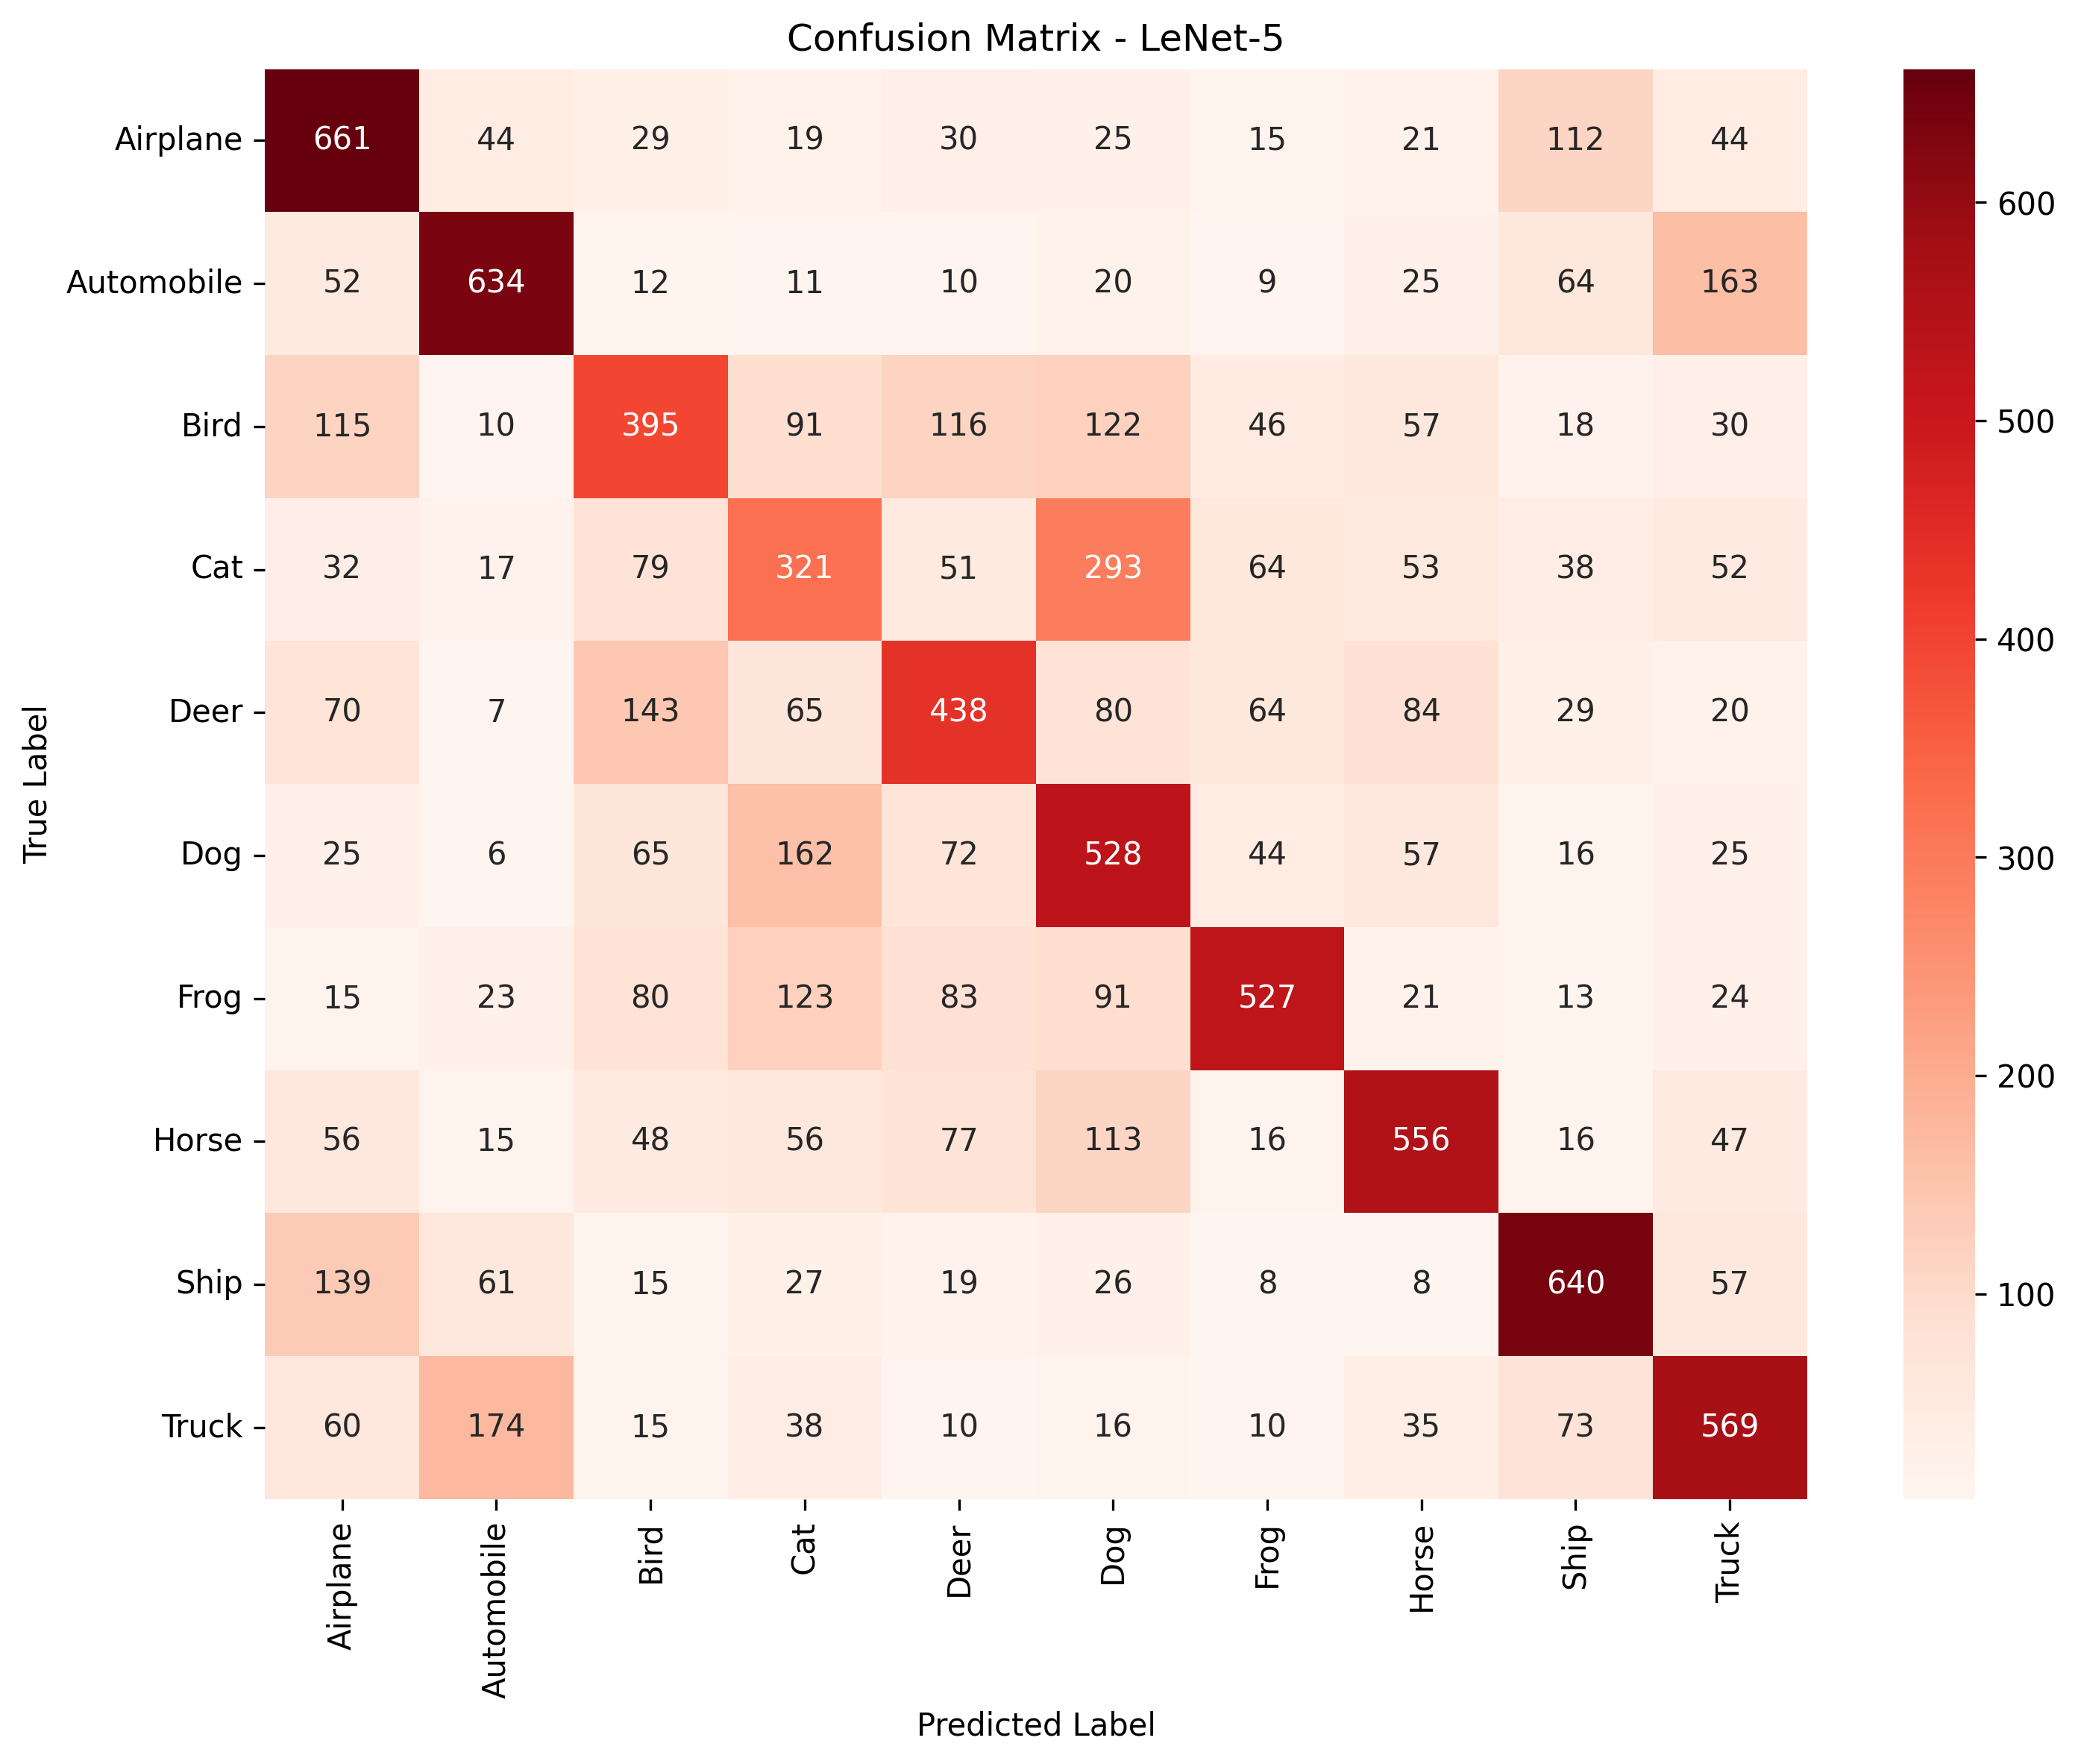
\includegraphics[width=0.7\textwidth]{plots/6e_confusion_matrix_lenet5.png}
\caption{Confusion Matrix -- LeNet-5}
\end{figure}

\noindent\textit{Inference:} As a shallow architecture trained entirely from scratch (no pretrained weights are available for LeNet-5), it achieves the lowest accuracy overall at 52.69\%, reflecting its limited capacity to capture complex features in a 10-class natural image dataset.

\begin{figure}[H]
\centering
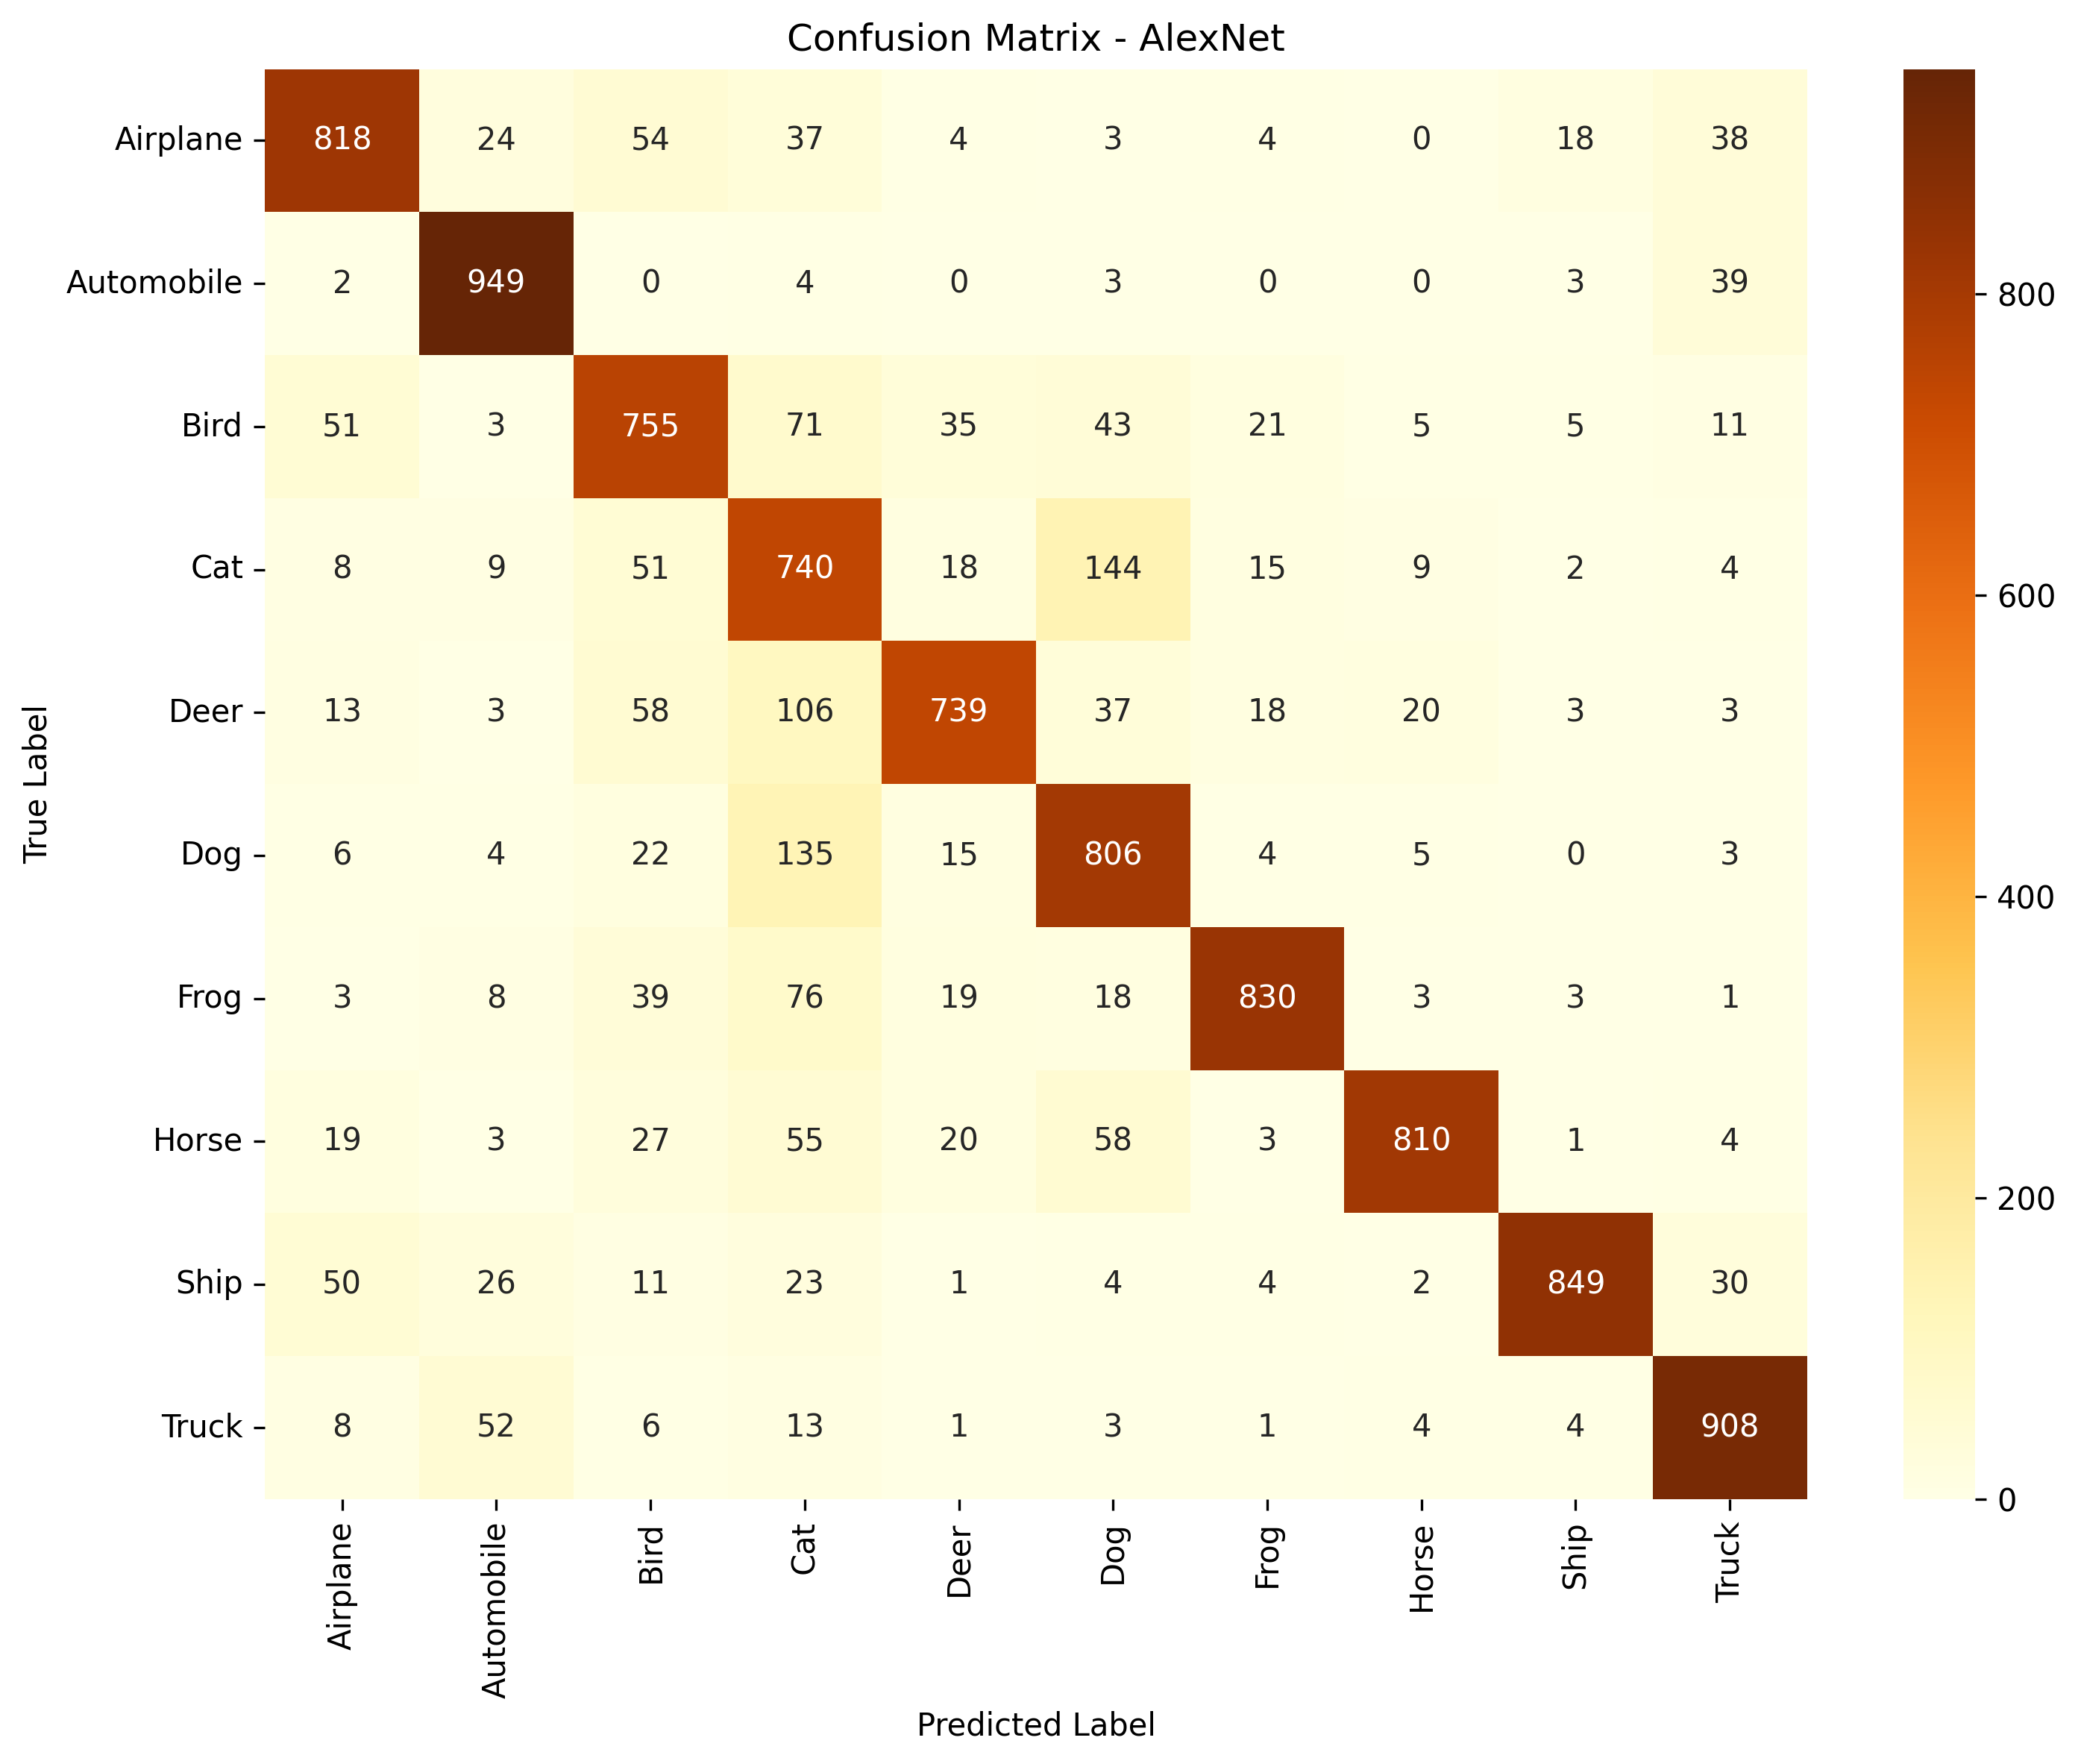
\includegraphics[width=0.7\textwidth]{plots/6f_confusion_matrix_alexnet.png}
\caption{Confusion Matrix -- AlexNet}
\end{figure}

\noindent\textit{Inference:} AlexNet, trained from scratch with Batch Normalization and Dropout, achieves the highest overall test accuracy (82.04\%) despite having no pretrained weights, showing that a well-regularized architecture matched to CIFAR-10's scale can outperform ImageNet-pretrained backbones whose native resolution mismatch limits transfer effectiveness.

\begin{figure}[H]
\centering
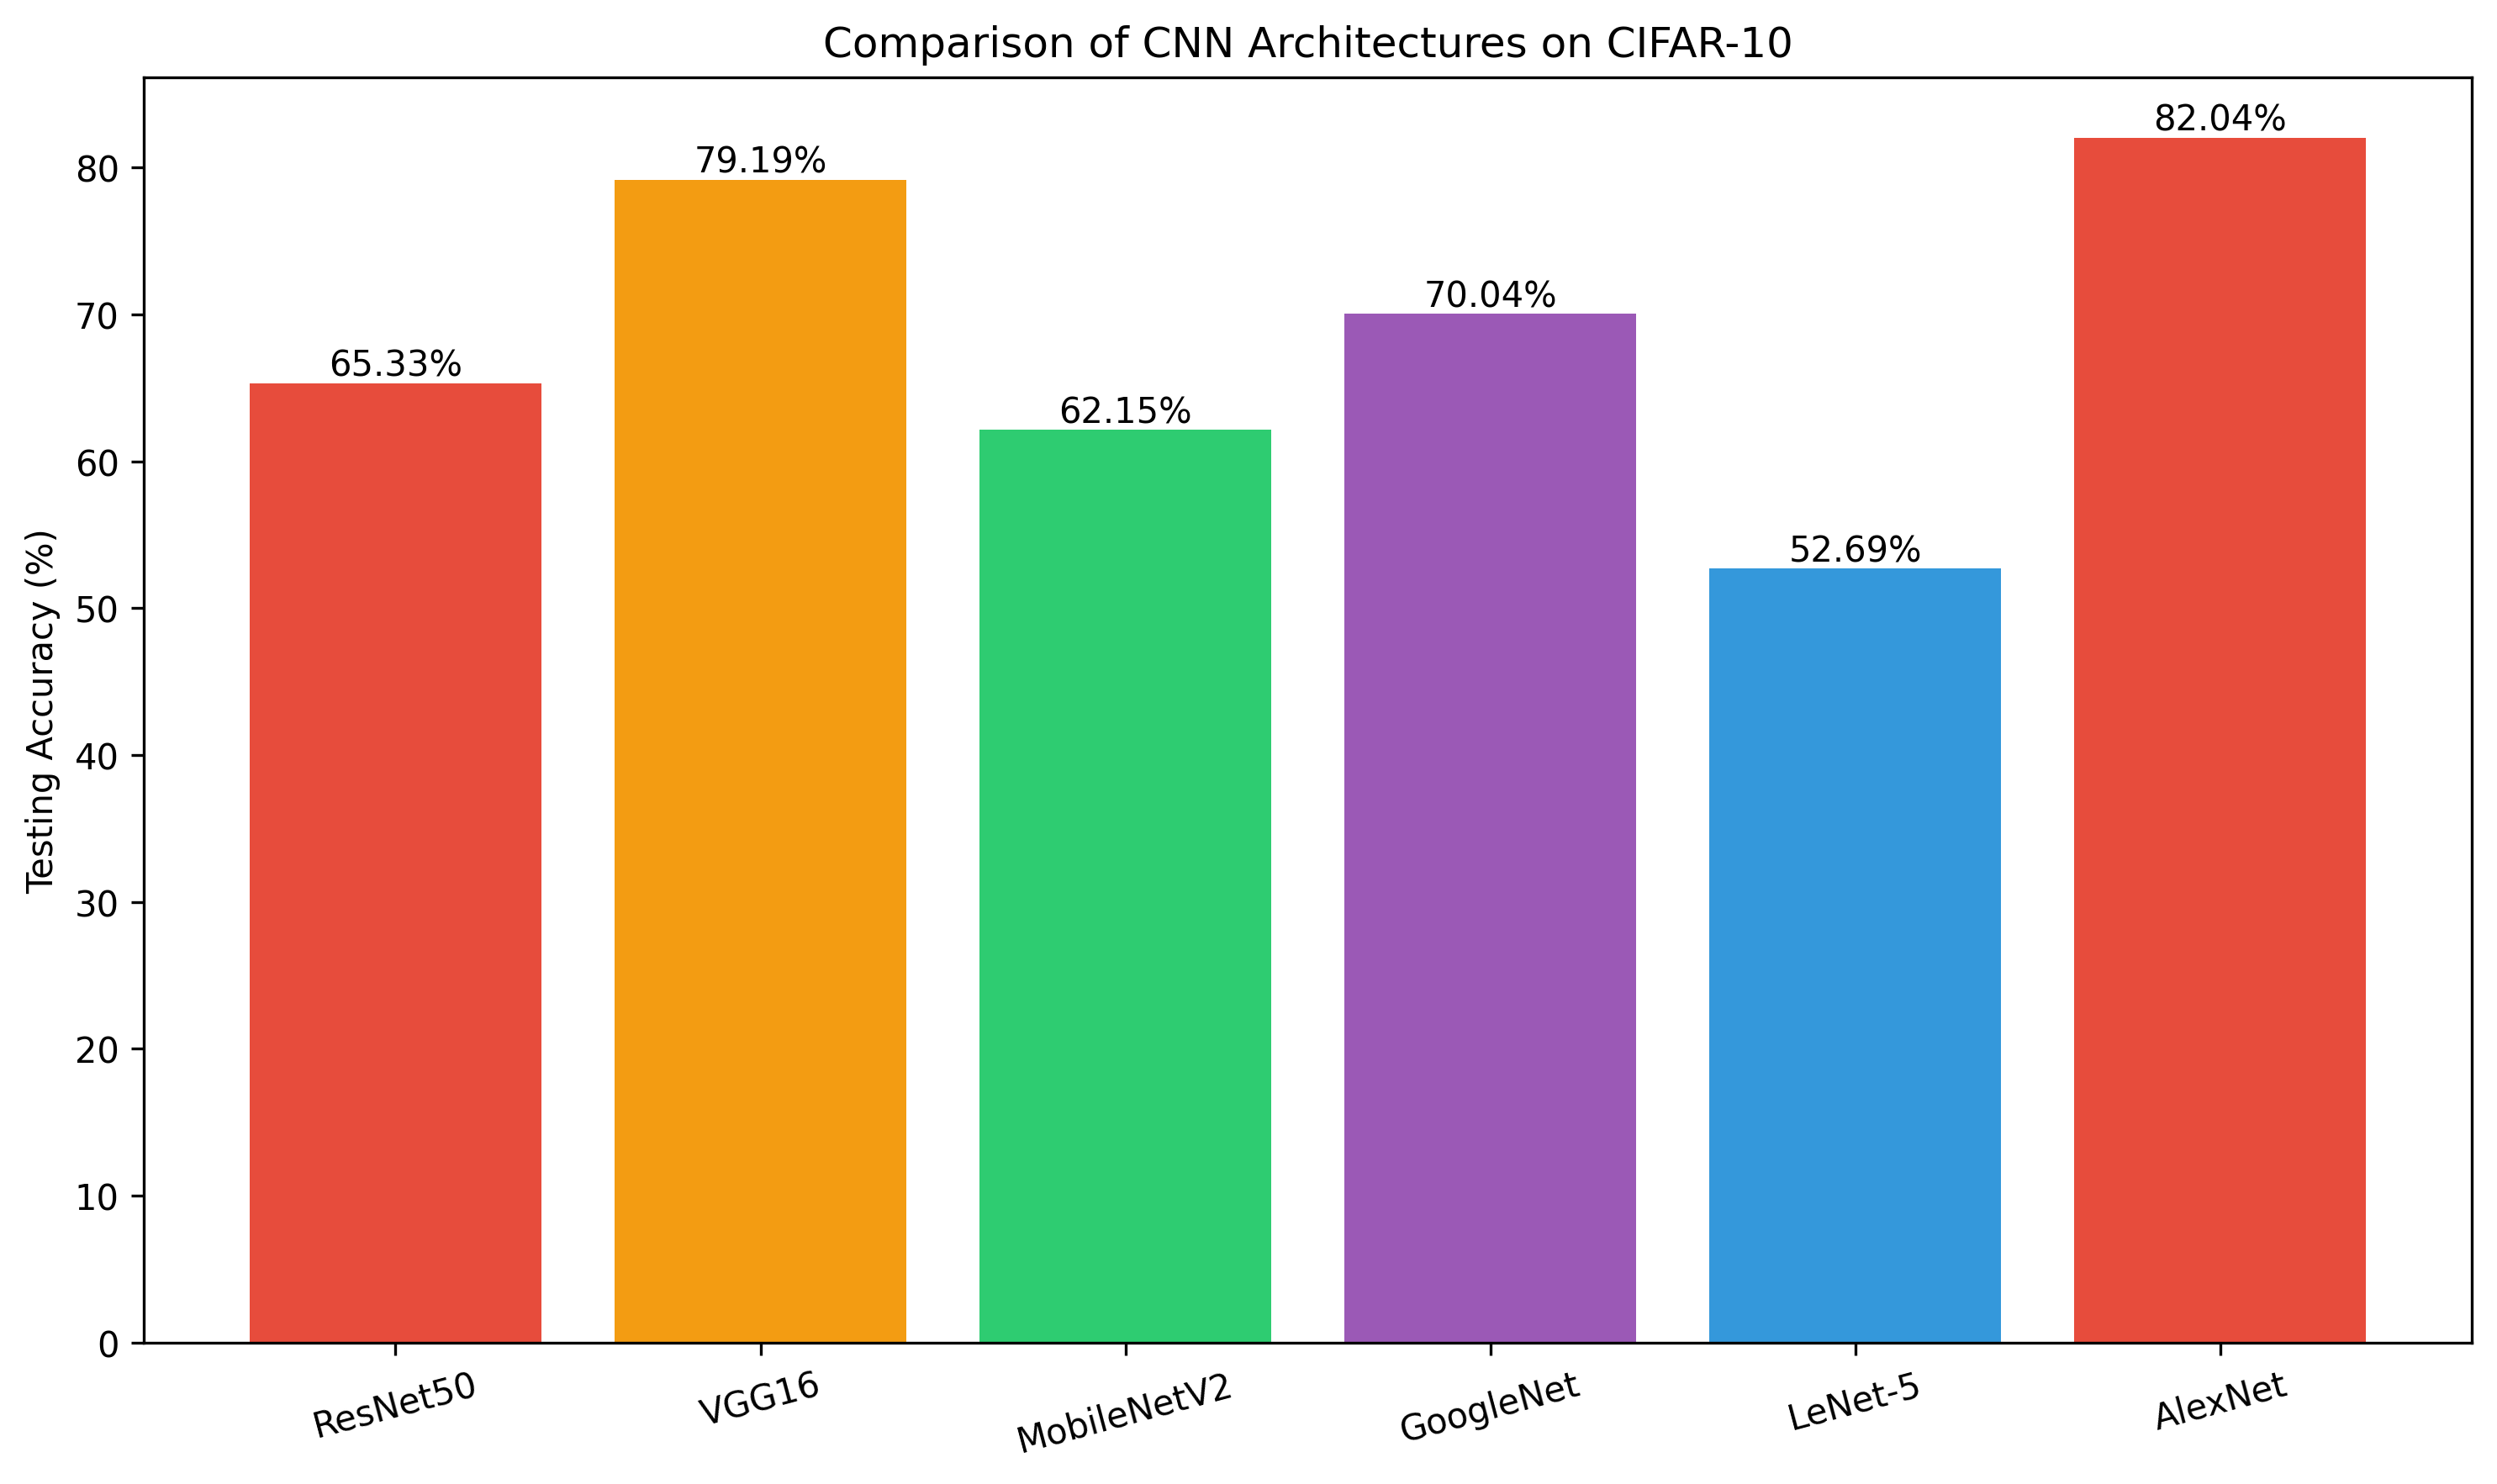
\includegraphics[width=0.75\textwidth]{plots/8_model_comparison_accuracy.png}
\caption{Testing Accuracy Comparison Across All Five CNN Architectures}
\end{figure}

\noindent\textit{Inference:} AlexNet (82.04\%) and VGG16 (79.19\%) achieved the highest test accuracy on CIFAR-10, outperforming the deeper ResNet50 (65.33\%) and InceptionV3 (70.04\%). This suggests that, for a small $32\times32$ dataset with limited fine-tuning epochs, architectures adapted/trained closer to the target input scale can outperform larger ImageNet-pretrained backbones whose learned features are optimized for $224\times224$ inputs.

%%%%%%%%%%%%%%%%%%%%%%%%%%%%%%%%%%%%%%%%%%%%%%%%%%%%%%%%%%%%

\section*{18. Results}

\subsection*{18.1 Performance Metrics}

\begin{center}

\begin{tabular}{|p{5cm}|p{4cm}|}

\hline

Metric & Value\\

\hline

Training Accuracy & 98.90\%\\

\hline

Testing Accuracy & 65.33\%\\

\hline

Precision & 65.35\%\\

\hline

Recall & 65.33\%\\

\hline

F1-score & 65.30\%\\

\hline

Training Time & 6.18 minutes\\

\hline

Total Parameters & 24,114,826\\

\hline

\end{tabular}

\end{center}

\vspace{5mm}

\subsection*{18.2 Comparison of CNN Architectures}

\begin{center}

\begin{tabular}{|l|c|c|c|}

\hline

Model &
Parameters &
Accuracy (\%) &
Training Time\\

\hline

LeNet-5 & 83,126 & 52.69 & 1.83 min\\

\hline

AlexNet & 5,282,378 & 82.04 & 4.87 min\\

\hline

VGG16 & 14,848,586 & 79.19 & 6.49 min\\

\hline

GoogleNet & 22,329,898 & 70.04 & 11.15 min\\

\hline

ResNet50 & 24,114,826 & 65.33 & 6.18 min\\

\hline

\end{tabular}

\end{center}

%%%%%%%%%%%%%%%%%%%%%%%%%%%%%%%%%%%%%%%%%%%%%%%%%%%%%%%%%%%%

\section*{19. Discussion Questions}

Answer the following questions.

\begin{enumerate}

\item Why is AlexNet considered a breakthrough in deep learning?

\textit{Answer:} AlexNet (2012) was the first deep CNN to win ImageNet by a large margin. It proved that deep networks could be trained efficiently on GPUs, and it popularised ReLU activation (faster convergence than sigmoid/tanh), Dropout (reduces overfitting), and data augmentation -- ideas that became standard in nearly all later architectures.

\item Why does VGG16 use only $3\times3$ convolution filters?

\textit{Answer:} Stacking multiple $3\times3$ filters gives the same effective receptive field as a larger filter (e.g. two $3\times3$ layers $\approx$ one $5\times5$) while using fewer parameters and adding an extra non-linearity (ReLU) between them, which improves feature discrimination and keeps the network simpler to design.

\item Explain the advantages of the Inception module.

\textit{Answer:} The Inception module applies multiple filter sizes ($1\times1$, $3\times3$, $5\times5$) and pooling in parallel and concatenates their outputs, capturing features at multiple scales in a single layer. The $1\times1$ convolutions before larger filters reduce dimensionality first, cutting computation and parameters while keeping accuracy high.

\item What is the purpose of residual learning?

\textit{Answer:} Residual learning lets a layer learn only the residual $F(x) = H(x) - x$ instead of the full mapping $H(x)$, with the output computed as $F(x)+x$ via a skip connection. This allows gradients to flow directly through the identity path, solving the vanishing-gradient problem and enabling much deeper networks to be trained successfully.

\item Differentiate LeNet and ResNet.

\textit{Answer:} LeNet-5 (1998) is a shallow 7-layer network with $\sim$60K parameters, using average pooling and tanh activations, designed for small grayscale digit images. ResNet50 (2015) is a 50-layer deep network with $\sim$25.6M parameters, using residual/skip connections and ReLU, capable of learning much richer hierarchical features from large-scale natural images. In our experiment this showed up directly: LeNet-5 reached only 52.69\% test accuracy on CIFAR-10 versus ResNet50's much larger capacity, though ResNet50's transfer-learning accuracy (65.33\%) was still limited here by the small $32\times32$ input.

\item What is Transfer Learning?

\textit{Answer:} Transfer learning reuses a CNN already pretrained on a large dataset (e.g. ImageNet) for a new, related task. Instead of training from scratch, the pretrained convolutional base (which has already learned general features like edges and textures) is reused, its classifier head is replaced, and only the new layers (or a few unfrozen top layers) are trained on the new dataset -- reducing training time and data requirements.

\item Why is fine tuning required?

\textit{Answer:} With only the classifier head trained and the base frozen, the pretrained features may not be fully specialised to the new dataset. Fine tuning unfreezes the last few convolutional layers and trains them at a low learning rate, letting the network adapt its high-level features to the target data and typically improving accuracy further -- as seen in our ResNet50 run, where validation accuracy rose from 64.05\% to 65.33\% after fine tuning.

\item Explain the difference between dilated convolution and transpose convolution.

\textit{Answer:} Dilated (atrous) convolution inserts gaps between kernel elements to enlarge the receptive field without adding parameters or reducing spatial resolution -- useful for tasks like semantic segmentation. Transpose convolution does the opposite job: it performs learnable upsampling to increase the spatial size of a feature map, commonly used in autoencoders, GANs, and image generation.

\item Why do pretrained models converge faster?

\textit{Answer:} Pretrained models start with weights that already encode general-purpose visual features (edges, textures, shapes) learned from a large dataset like ImageNet, rather than random weights. This gives training a strong starting point, so fewer epochs are needed to reach good performance compared to training from scratch. This was visible in our results: the transfer-learning models (ResNet50, VGG16, MobileNetV2, GoogleNet) reached high training accuracy within just a few epochs, though full generalisation to CIFAR-10's small $32\times32$ images was still limited.

\item Compare the computational complexity of LeNet and ResNet.

\textit{Answer:} LeNet-5 is extremely lightweight ($\sim$60K--83K parameters in our implementation), with only two convolution layers, making it fast to train but limited in representational power. ResNet50 is far more complex (24.1M parameters, 50 layers), requiring significantly more computation and memory per forward/backward pass. This matched our timing results: LeNet-5 trained in 1.83 minutes versus ResNet50's 6.18 minutes for a comparable number of epochs.

\end{enumerate}

%%%%%%%%%%%%%%%%%%%%%%%%%%%%%%%%%%%%%%%%%%%%%%%%%%%%%%%%%%%%

\section*{20. Additional Exercises}

\begin{enumerate}

\item Implement transfer learning using VGG16.

\item Repeat the experiment using ResNet50.

\item Compare Adam and SGD optimizers.

\item Compare training with frozen layers and fine tuning.

\item Evaluate the model using Precision, Recall and F1-score.

\item Compare the performance of LeNet, AlexNet and ResNet.

\end{enumerate}

%%%%%%%%%%%%%%%%%%%%%%%%%%%%%%%%%%%%%%%%%%%%%%%%%%%%%%%%%%%%

\section*{21. References}

\begin{enumerate}

\item Yann LeCun, Leon Bottou, Yoshua Bengio and Patrick Haffner,
\emph{Gradient-Based Learning Applied to Document Recognition},
Proceedings of the IEEE, 1998.

\item Alex Krizhevsky, Ilya Sutskever and Geoffrey Hinton,
\emph{ImageNet Classification with Deep Convolutional Neural Networks},
NeurIPS, 2012.

\item Karen Simonyan and Andrew Zisserman,
\emph{Very Deep Convolutional Networks for Large-Scale Image Recognition},
ICLR, 2015.

\item Christian Szegedy et al.,
\emph{Going Deeper with Convolutions},
CVPR, 2015.

\item Kaiming He, Xiangyu Zhang, Shaoqing Ren and Jian Sun,
\emph{Deep Residual Learning for Image Recognition},
CVPR, 2016.

\item Ian Goodfellow, Yoshua Bengio and Aaron Courville,
\emph{Deep Learning},
MIT Press, 2016.

\item TensorFlow Documentation:
\url{https://www.tensorflow.org}

\item Keras Documentation:
\url{https://keras.io}

\end{enumerate}

%%%%%%%%%%%%%%%%%%%%%%%%%%%%%%%%%%%%%%%%%%%%%%%%%%%%%%%%%%%%

\end{document}